% !TeX root = ../main.tex
%\chapter{The LHC and ATLAS Experiment}

The research detailed in this thesis relies on data gathered by the ATLAS experiment at the Large Hadron Collider (LHC). This chapter presents an overview of the LHC's design, operational history, and future roadmap, accompanied by a fundamental introduction to collider physics. Following this, the chapter offers an in-depth review of the ATLAS detector, highlighting the architecture, calibration, performance metrics, and scheduled upgrades for its various sub-detectors. The primary design specifications can be found in the ``design'' column of Table~\ref{tab:LHCrun2param}.

%-------------LHC----------------
\section{The Large Hadron Collider}

Recognized globally as the most massive and potent particle accelerator ever constructed, the Large Hadron Collider (LHC) operates roughly 100 meters below ground near Geneva, straddling the Franco–Swiss border~\cite{Evans:2008zzb}. The European Organization for Nuclear Research (CERN) spearheaded its design and construction, supported by substantial contributions from Japan and the United States.

Illustrated in Figure~\ref{fig:CERNAccComplex}, the CERN accelerator complex~\cite{CERNAccComplex} functions as a massive, interconnected network of accelerators designed to progressively ramp up the energy of proton beams prior to entering the main LHC ring. The acceleration pipeline kicks off at Linac4, acting as the initial provider of proton beams. Here, negative hydrogen ions ($H^-$) undergo an initial acceleration to 160~MeV by Linac4 before being transferred into the Proton Synchrotron Booster (PSB). Upon entering the PSB, these hydrogen ions are stripped of their electrons. The remaining bare protons are subsequently boosted to an energy level of 2~GeV.

Following this, the proton beam is routed to the Proton Synchrotron (PS) to be accelerated to 26~GeV, and it is then passed to the Super Proton Synchrotron (SPS). At this stage, the beam energy is pushed up to 450~GeV. From the SPS facility, the protons are injected directly into the LHC's dual beam pipes, causing one beam to travel clockwise and the second to travel counterclockwise. It takes approximately 20 to 25 minutes for these beams to achieve their operational collision energy, which is 6.8~TeV per beam for Run~3 (and was 6.5~TeV during Run~2).

A comparable acceleration strategy is utilized for heavy-ion beams. Lead ions are generated at Linac3, after which they are accumulated and accelerated using the Low Energy Ion Ring (LEIR). Once extracted from LEIR, these ions travel through the PS, the SPS, and ultimately enter the LHC, echoing the trajectory of the proton beams. Both heavy-ion and proton beams are deliberately engineered to intersect and collide at four distinct interaction points distributed around the LHC ring.

\begin{figure}[!htbp]
    \centering
    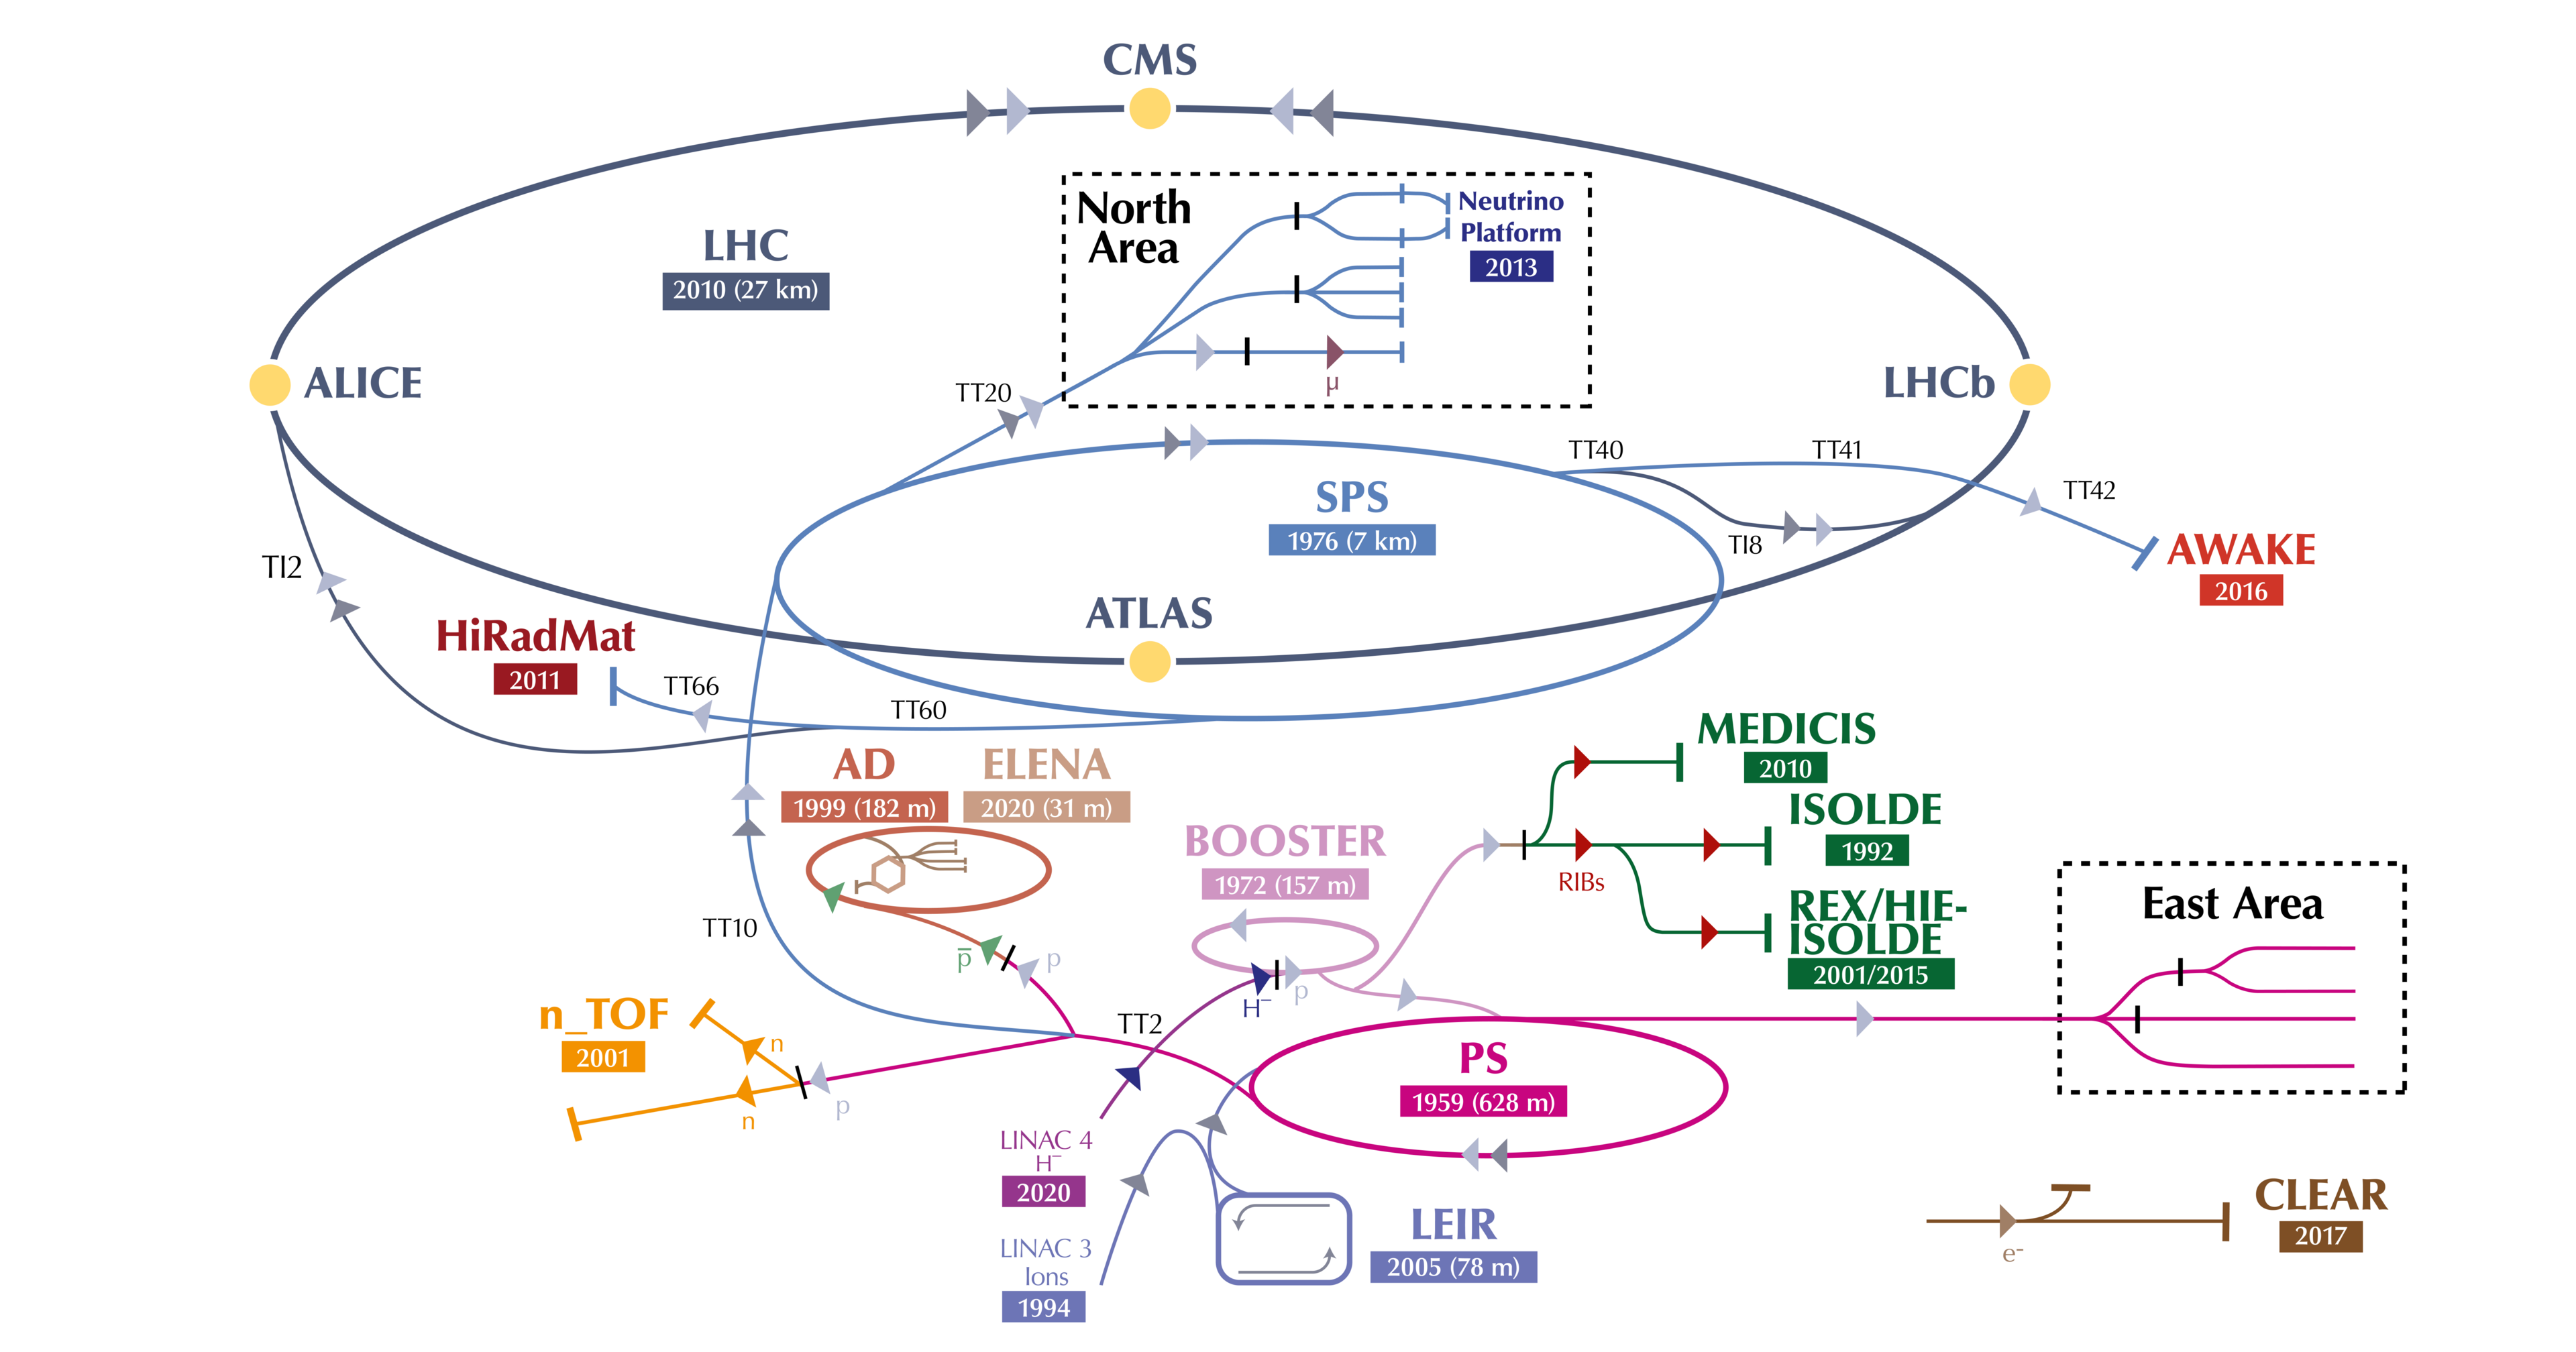
\includegraphics[width=0.95\linewidth]{figures/ch3-LHC-ATLAS/CERN_accelerator_complex_2022.png}
    \caption{The CERN accelerator complex.}
    \label{fig:CERNAccComplex}
\end{figure}

Spanning 27 kilometers, the LHC is a circular accelerator that employs a combination of radiofrequency (RF) cavities and superconducting magnets to boost the energy of the circulating charged particles. The two opposing particle beams are housed in isolated beam pipes, which are kept at an ultrahigh vacuum approaching $10^{-6}~\text{mbar}$. A massive array of superconducting magnets steers and stabilizes the beams along the circular trajectory. This includes 1,232 dipole magnets responsible for bending the particle paths, 392 quadrupole magnets dedicated to focusing them, and specialized magnets designed to compress the beams into microscopic dimensions immediately prior to collision. Furthermore, the RF cavities serve to accelerate the particles, magnifying their energy by a factor of roughly 14 compared to their initial injection energy.

Within this accelerator, the paired high-energy beams—comprising either lead ions or protons—travel in contrary directions at velocities approaching the speed of light. Collisions between these beams are orchestrated at four specific interaction points, with a major detector experiment stationed at each. These four prominent detector collaborations are ATLAS~\cite{ATLAS2008}, CMS~\cite{CMS2008}, ALICE~\cite{ALICE2008}, and LHCb~\cite{LHCb2008}. Both CMS and ATLAS act as general-purpose detectors aimed at executing high-precision measurements of Standard Model phenomena and hunting for novel physics beyond the Standard Model. Conversely, ALICE is tailored for heavy-ion collisions to investigate the quark–gluon plasma formed under conditions of extreme density and temperature, whereas LHCb is dedicated to analyzing CP violation and beauty-hadron decays within the heavy-flavor domain.

%%%%%%%%%%%%%%%
Beam energy and luminosity stand out as the most critical accelerator parameters. Elevated beam energies permit collisions to investigate much smaller distance scales by probing shorter wavelengths, thereby unlocking the ability to study the deeper fundamental structures of matter. Meanwhile, a higher luminosity yields a greater volume of collision events, which amplifies the sensitivity to infrequent processes and drastically boosts the likelihood of novel discoveries. For modern accelerators, the standard energy unit is the $10^{12}$ electron-volt (TeV). 
Luminosity can be conceptualized as a measure of the particle beams' ``intensity.'' The instantaneous luminosity ($L$) quantifies the collision rate per unit of time across a unit of cross-sectional area, mathematically expressed as:
\begin{equation}
    L = \frac{f n_1 n_2}{A},
\end{equation}
where $f$ denotes the revolution frequency of the particle bunches, while $n_1$ and $n_2$ represent the number of particles contained in each colliding bunch. The parameter $A$ signifies the effective transverse cross-sectional area shared by the beams. In contrast, the integrated luminosity ($\int L\,dt$) characterizes the cumulative luminosity supplied over a specified duration. This metric is crucial for calculating the total expected number of events for a given physical process over that period:
\begin{equation}
    N_{\text{event}} = \sigma \times \int L \,dt .
\end{equation}
In this formula, $\sigma$ represents the cross-section, 
which quantifies the probability of a specific reaction occurring between the interacting particles. The conventional unit for measuring cross-section is the barn (b), defined as $1~\text{b} = 10^{-24}~\text{cm}^2$.

%%%%%%%%%%%%%%%
A comprehensive timeline detailing the LHC's operational history and key milestones—spanning from Run~1 to Run~3, alongside the scheduled long shutdown phases—is provided in Table~\ref{tab:lhc_timeline}. Additionally, Table~\ref{tab:LHCrun2param} compares the primary theoretical design parameters of the LHC with the actual operational values recorded throughout the Run~2 data-taking period. The analyses discussed throughout this thesis heavily depend on the dataset accumulated during Run~2.

\vspace*{0.5cm}
\begin{table}[htbp]
  \centering
  \caption{Timeline of LHC operations and major milestones.}
  \label{tab:lhc_timeline}
  \begin{tabular}{p{3.2cm} p{3.2cm} p{8.0cm}}
    \hline
    \textbf{Phase} & \textbf{Period} & \textbf{Description} \\
    \hline
    Run~1 & 2010--2013 &
    Initial physics operation with proton--proton collisions at 3.5~TeV per beam (7~TeV center-of-mass) in 2010--2011, increasing to 4~TeV per beam (8~TeV center-of-mass) in 2012. The Higgs boson was discovered in 2012. \\

    Long Shutdown~1 (LS1) & 2013--2014 &
    Maintenance and consolidation of the superconducting magnet system, enabling safe operation at higher beam energies. \\

    Run~2 & 2015--2018 &
    Operation at 6.5~TeV per beam (13~TeV center-of-mass), significantly enhancing sensitivity to physics beyond the Standard Model. \\

    Long Shutdown~2 (LS2) & 2019--2021 &
    Major upgrades in preparation for Run~3, including improvements to the injector complex to increase beam intensity and luminosity. \\

    Run~3 & 2022--2026 &
    Physics operation began in July 2022 at a record energy of 6.8~TeV per beam (13.6~TeV center-of-mass). The run is extended to early 2026 to maximize data collection prior to Long Shutdown~3. \\

    Long Shutdown~3 (LS3) & 2026+ &
    Preparation for the High-Luminosity LHC (HL-LHC) era, targeting a substantial increase in delivered integrated luminosity. \\

    Run~4 and beyond  & 2030+ &
    High-luminosity operations targeting more than $3000~\text{fb}^{-1}$ of total integrated luminosity. \\ 

    \hline
  \end{tabular}
\end{table}

\vspace*{0.5cm}
\begin{table}[htbp]
\centering
\caption{LHC operation parameters for the Run-2 data-taking period.}
\label{tab:LHCrun2param}
\begin{tabular}{ l | c || c | c | c | c}
\hline
 \textbf{Parameter} & \textbf{Design} & \textbf{2018} & \textbf{2017} & \textbf{2016} & \textbf{2015} \\
 \hline
 Energy [TeV] & 7.0 & 6.5 & 6.5 & 6.5 & 6.5 \\
 Number of bunches & 2808 & 2556 & 2556-1868 & 2220 & 2244 \\
 Number of bunches per train & 288 & 144 & 144-128 & 96 &  144 \\
 Max. energy per beam [MJ] & 362 & 312 & 315 & 280 & 280 \\
 $\beta^*$ & 55 & 25-30 & 30-40 & 40 & 80 \\
 Protons per bunch [$10^{11}$] $N_b$ & 1.15 & 1.1 & 1.25 & 1.25 & 1.2 \\
 Normalized emittance $\epsilon_n$ & 3.75 & 1.8-2.2 & 1.8-2.2 & 1.8-2 & 2.6-3.5 \\
 Peak luminosity [$10^{34} \textrm{cm}^{-2} \textrm{s}^{-1}$] & 1.0 & 2.1 & 2 & 1.5  & <0.6 \\
 Half crossing angle [$\mu$rad] & 142.5 & 130-150    & 120-150 & 140-185 & 185 \\
\hline
\end{tabular}
\end{table}


\subsection{High-Luminosity LHC Upgrade}

A crucial metric for evaluating an accelerator's performance is its luminosity, which directly correlates with the frequency of collisions within a specific timeframe. As luminosity increases, experimental collaborations can harvest significantly larger datasets, facilitating the observation and analysis of extremely rare physical processes.

Set to commence operations in 2030 and continue for the foreseeable future, the High-Luminosity Large Hadron Collider (HL-LHC) represents a massive upgrade to the current facility. The HL-LHC target entails delivering an unprecedented instantaneous luminosity of $L = 7.5 \times 10^{34}~\text{cm}^{-2}\text{s}^{-1}$. Coupled with an expected annual integrated luminosity of roughly $250~\text{fb}^{-1}$, the project aims to compile a colossal final dataset ranging between $3000 - 4000~\text{fb}^{-1}$.
A visual representation of the comprehensive LHC roadmap is provided in Figure~\ref{fig:LHCroadmap}.

\vspace*{0.5cm}
\begin{figure}[!htbp]
    \centering
    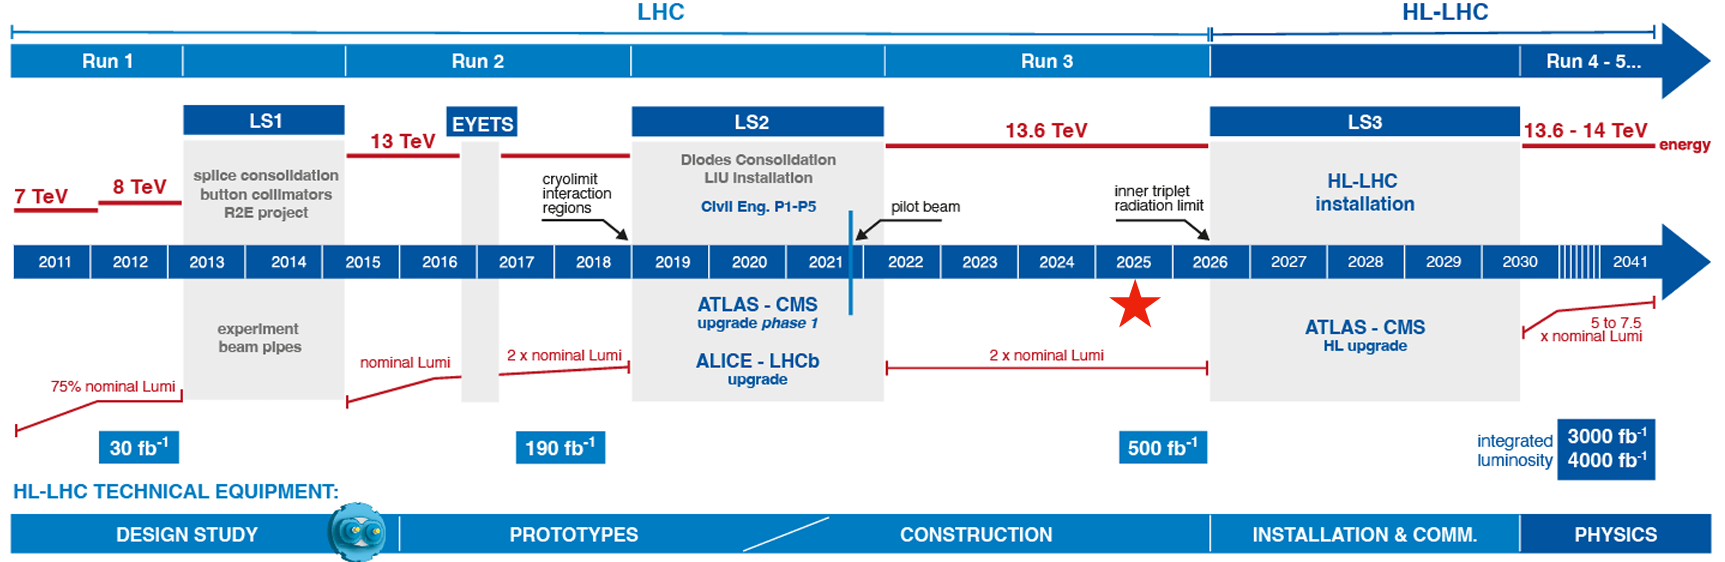
\includegraphics[width=0.95\linewidth]{figures/ch3-LHC-ATLAS/LHC-plan.png}
    \caption{The road map of the LHC.}
    \label{fig:LHCroadmap}
\end{figure}

Thanks to the HL-LHC, physicists will be empowered to scrutinize familiar Standard Model processes with unparalleled accuracy while simultaneously searching for exceedingly rare events that might hint at new physics. Most notably, the dramatic surge in luminosity will pave the way for exhaustive studies of the Higgs boson's characteristics. Projections indicate that the HL-LHC will yield no fewer than 15 million Higgs bosons annually, a staggering increase compared to the roughly three million generated by the LHC during the entirety of 2017.

A significant portion of the research undertaken for this PhD thesis focuses on the planned upgrade of the ATLAS Muon Spectrometer tailored for the HL-LHC era (detailed in Chapter~\ref{chap:sMDT}). This enhancement is absolute necessity to sustain optimal detector performance despite the drastically elevated particle rates and harsh radiation environment anticipated in the coming high-luminosity phase.


\section{Phenomenology of Collider Physics}

High-energy proton beams are collided at the LHC, generating a diverse array of final-state particles. As composite entities rather than point-like fundamental particles, protons are made up of gluons and quarks, jointly known as partons. The predominant physical interest in these high-energy proton–proton ($pp$) collisions stems from the interactions between partons occurring during inelastic hard-scattering events. These specific events feature substantial momentum transfers and can be accurately modeled using perturbative calculations, distinguishing them cleanly from softer, low-momentum-transfer interactions. A typical $pp$ collision event recorded at the LHC is mapped out in Figure~\ref{fig:LHCcollision}.
\begin{figure}[!htbp]
    \centering
    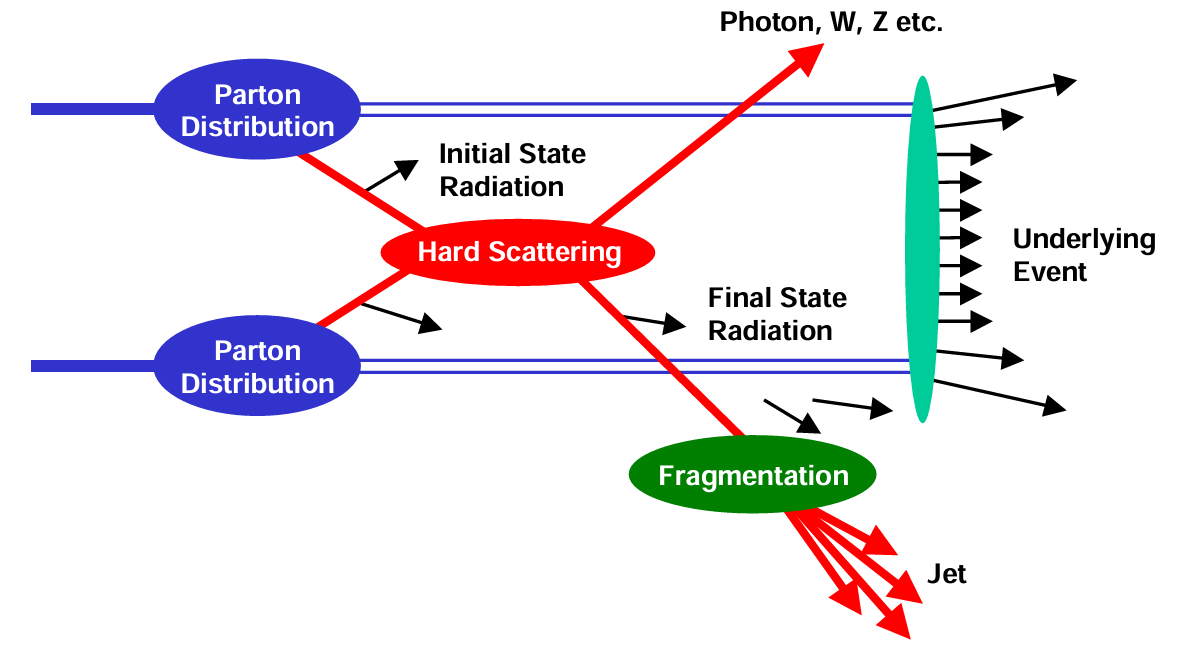
\includegraphics[width=0.8\linewidth]{figures/ch3-LHC-ATLAS/Hadron-collision.png}
    \caption{A representative $pp$ collision event at the LHC.}
    \label{fig:LHCcollision}
\end{figure}

Constructing a theoretical model for a $pp$ collision requires integrating several essential elements. Firstly, the probability distributions of partonic momentum inside a proton are modeled by parton distribution functions (PDFs)~\cite{CTEQ2016,NNPDF2017,PDF4LHC2015} at a specified factorization scale $\mu$.
Secondly, the hard-scattering mechanism—the core process exploited in hadron colliders like the LHC—dictates the short-distance dynamics and triggers the creation of massive particles, such as the Higgs boson. Following this initial hard interaction, the phenomena of jet fragmentation and hadronization~\cite{Andersson1983Lund,Webber1984Cluster} delineate how the resulting quarks and gluons transition into observable hadronic states. Additionally, final- and initial-state radiation models account for the supplementary emission of photons or gluons from the departing and approaching partons. Concurrently, the underlying event accounts for the multitude of secondary particles originating from the shattered remnants of the interacting protons.

\subsection{Cross-Section Calculation for Proton-Proton Collision Process}
\label{sec:cal-xs}

Figure~\ref{fig:hadron-coll} illustrates the cross-section computation framework for collisions between proton beams A and B.
\begin{figure}[!htbp]
    \centering
    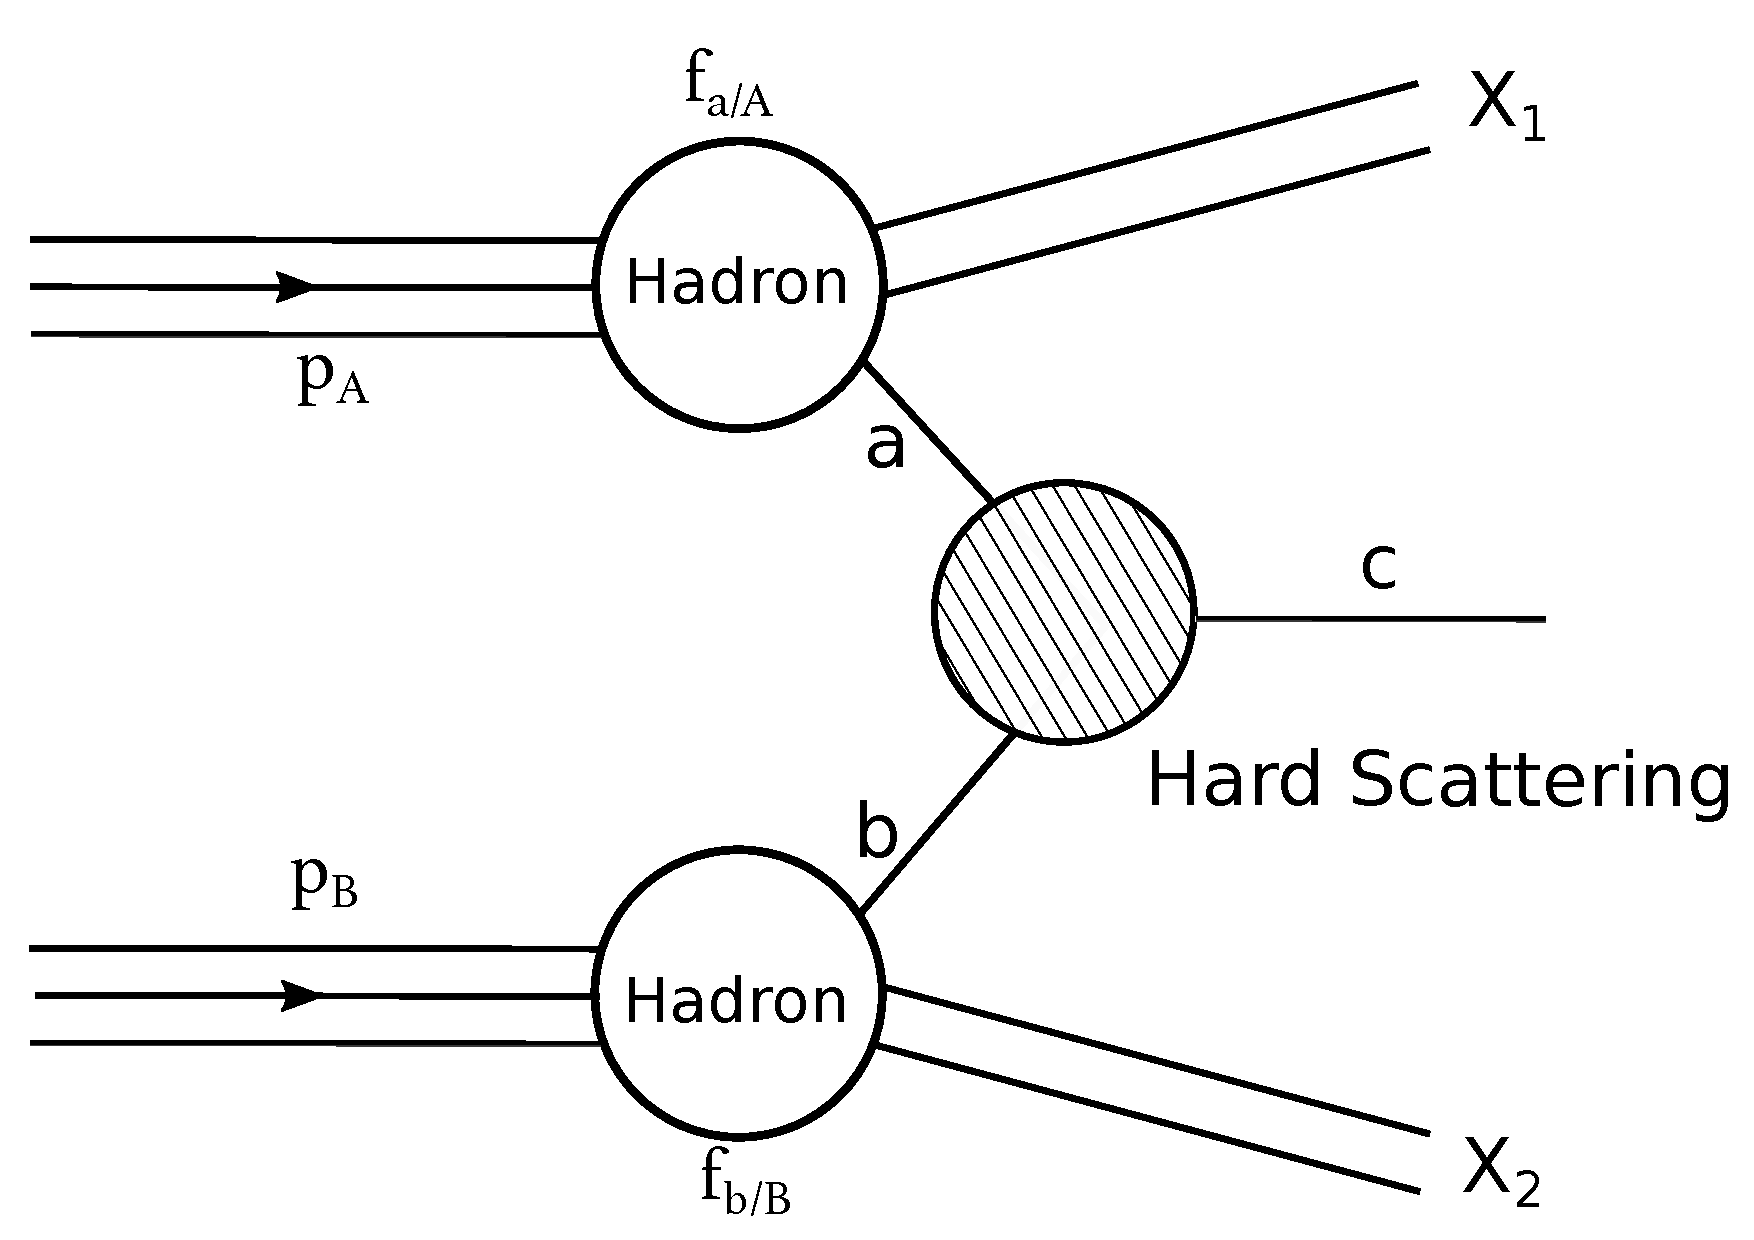
\includegraphics[width=0.5\linewidth]{figures/ch3-LHC-ATLAS/hadron_coll.pdf}
    \caption{The proton-proton collision process.}
    \label{fig:hadron-coll}
\end{figure}

\begin{equation}
    A + B \rightarrow C + X,
\end{equation}
In this expression, $X$ symbolizes the remnants left over from the incoming hadrons. When viewed strictly at the partonic hard-scattering level, the interaction is reduced to:
\begin{equation}
    a + b \rightarrow c.
\end{equation}
Within this paradigm, the variables $X_1$ and $X_2$ from Figure~\ref{fig:hadron-coll} represent the underlying events linked to the overall process.
To derive the comprehensive cross-section for such a proton-proton interaction, one must integrate over the momentum fractions $x_a$ and $x_b$, while summing across every permissible initial parton combination:
\begin{equation}
    \sigma(A + B \rightarrow C+X) = \sum_{a, b}
    \int_{0}^{1} \int_{0}^{1} dx_a dx_b f_{a/A}(x_a, Q^2) f_{b/B}(x_b, Q^2) 
    \sigma_{a+b \rightarrow c}
    ,
\end{equation}
where the variables $f_{a/A}(x_a, Q^2)$ and $f_{b/B}(x_b, Q^2)$ denote the PDFs describing the momentum fractions $x_a$ and $x_b$ for partons $a$ and $b$, evaluated at a specific momentum transfer scale $Q^2$.

Calculations for production cross-sections in hadronic collisions rely heavily on the principles of perturbative quantum chromodynamics (pQCD). By incorporating higher-order corrections derived from perturbative expansions, the precision of these theoretical calculations is greatly enhanced.

For a specific process $pp \to X$ at the LHC, the inclusive cross-section evaluated up to the $n$-th order in perturbation theory is formulated as
\begin{equation}
    \sigma^{(n)}_{\text{inclusive}} 
    = 
    \sum_{a,b} \int_{0}^{1} dx_1 \int_{0}^{1} dx_2 \, f_{a}(x_1,\mu_F) f_{b}(x_2,\mu_F) \hat{\sigma}_{ab}^{(n)}(x_1,x_2,\mu_R,\mu_F),
\end{equation}
where $f_a(x,\mu_F)$ and $f_b(x,\mu_F)$ represent the parton distribution functions assessed at a specific factorization scale $\mu_F$ and momentum fraction $x$~\cite{Collins1989Factorization}. Additionally, $\hat{\sigma}_{ab}^{(n)}$ acts as the partonic cross-section associated with partons $a$ and $b$ computed to the $n$-th order, and $\mu_R$ serves as the renormalization scale~\cite{Ellis1996QCD}.

The exact partonic cross-section $\hat{\sigma}_{ab}$ can be expanded perturbatively as a power series in the strong coupling constant $\alpha_S$:
\begin{equation}
\hat{\sigma}_{ab}
=
\hat{\sigma}_{ab}^{(0)}
+
\alpha_S\,\hat{\sigma}_{ab}^{(1)}
+
\cdots
+
\alpha_S^{n}\hat{\sigma}_{ab}^{(n)}
+
\mathcal{O}(\alpha_S^{n+1}),
\end{equation}
where the baseline $\hat{\sigma}_{ab}^{(0)}$ signifies the leading-order (LO) component. The successive terms capture the next-to-leading order (NLO), next-to-next-to-leading order (NNLO), and subsequent higher-level perturbative corrections.

To compute production cross-sections—both across the full phase space and within the bounded experimental fiducial phase space—physicists employ Monte Carlo (MC) event generators rooted in pQCD frameworks. These advanced generators simulate the intricacies of hard-scattering events, the mechanics of parton showering~\cite{AltarelliParisi1977} (which tracks the pQCD-driven radiation of gluons and quarks prior to hadronization), and the ultimate hadronization phase that forms the observable jets.

%%%%%%%%%%%%%%%%%%%%
\subsection{The Diboson $\text{ZZ}$ Production Cross-Section at the LHC}% ZZ Production at LHC
\label{sec:zz-matrix-xs}

A central focus of this doctoral work is measuring the production cross-section of $\text{ZZ}$ boson pairs. To derive the relevant theoretical predictions, the Monte Carlo event generators \textsc{Matrix}~\cite{Grazzini2018MATRIX} and \textsc{Sherpa}~\cite{Gleisberg2009Sherpa} are utilized.

At the most basic (lowest) order, the generation of $\text{Z}$ boson pairs occurs either through the annihilation of a quark and an antiquark ($q\bar{q}$) or by means of gluon-gluon fusion operating across a closed quark loop.
Figure~\ref{fig:zz-prod} displays the lowest-order Feynman diagrams that dictate the primary pathways for $\text{ZZ}$ diboson generation at the LHC. Crucially, these diagrams highlight a core characteristic of the Standard Model: the strict absence of neutral triple gauge couplings, such as $\text{ZZZ}$ and $\text{ZZ}\gamma$, as explicitly demonstrated in Figure~\ref{fig:zz-prod}(c).
\begin{figure}[!htbp]
    \centering
    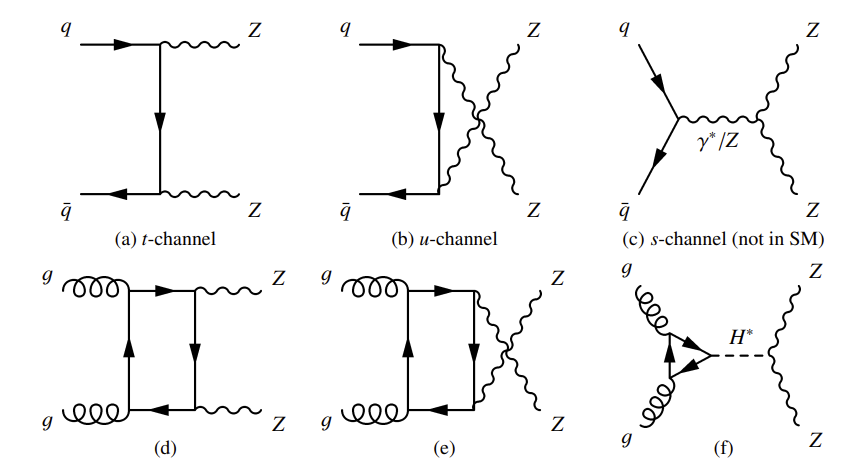
\includegraphics[width=0.8 \textwidth]{figures/ch3-LHC-ATLAS/ZZ-production-diagram.png}
    % \caption{Lowest-order Feynman diagrams of $\text{ZZ}$ production at the LHC. The (a) $t$-channel and (b) $u$-channel diagrams contribute to the $\text{ZZ}$ production cross-section, while the (c) 
    % $s$-channel diagram is not present in the SM due to the neutral $\text{ZZZ}$ or $\text{ZZ}\gamma$ vertex. Examples of one-loop contributions to $\text{ZZ}$ production from gluon pairs are shown in (d), (e), and (f).}
    \caption{Primary Feynman diagrams illustrating $\text{ZZ}$ generation at the LHC. Contributions to the overall cross-section arise from the $t$-channel (a) and $u$-channel (b) processes. Conversely, the Standard Model forbids the $s$-channel mechanism (c) because neutral $\text{ZZZ}$ and $\text{ZZ}\gamma$ vertices do not exist. Subfigures (d), (e), and (f) depict representative one-loop gluon-gluon fusion pathways.}
    \label{fig:zz-prod}
\end{figure}

Highly accurate theoretical estimates are generated via the \textsc{Matrix} framework, a versatile parton-level MC generator. \textsc{Matrix} excels at computing both total and fiducial cross-sections, alongside differential distributions, achieving next-to-next-to-leading order (NNLO) precision for QCD processes and next-to-leading order (NLO) precision for electroweak corrections. Throughout the ensuing sections, all theoretical modeling leverages the NNPDF3.0NNLO parton distribution functions~\cite{Ball2015NNPDF30}, adopting a strong coupling constant of $\alpha_S = 0.118$. 
Because \textsc{Matrix} integrates all valid leptonic decay branches for vector bosons—accounting perfectly for off-shell dynamics and spin correlations through non-resonant and resonant Feynman diagrams—it allows researchers to apply realistic fiducial cuts directly to the simulated leptonic final states.
For the specific $\text{ZZ}$ cross-section analysis performed in ATLAS, the defining cuts for the fiducial phase space, based on MC truth-level particles, are specified as follows:
\begin{itemize}
\item The kinematic variables of charged leptons ($\ell = e, \mu$) are ``dressed.'' This is achieved by combining the lepton's four-momentum with the momenta of any photons residing within a tight angular proximity of $\Delta R(\ell, \gamma) < 0.1$. In the absence of such photons, the lepton momentum is left unaltered;
\item The rapidity of all charged leptons must fall within the boundary $|{\eta}^{\ell} | < 2.5$;
\item A transverse momentum threshold is strictly enforced: $p_{\text{T}}^{\ell} > 30 (20)~\text{GeV}$ for the primary (secondary) charged lepton; 
\item The invariant mass of the dilepton pair is constrained to the window: $76 < m_{\ell\ell} < 106~\text{GeV}$;
\item The missing transverse energy, attributed to escaping neutrinos, must exceed $E_{\text{T}}^{\text{miss}} > 95~\text{GeV}$; % reco > 110
\item The angular distance separating the charged leptons is capped at $\Delta R_{\ell\ell} < 1.8$;  % reco-level < 1.8)
\item The azimuthal angle divergence between the two Z bosons must satisfy $\Delta \Phi (E_{\text{T}}^{\text{miss}}, p_{\text{T}}^{\ell\ell}) > 2.2$;  % reco is >2.7
\item The fraction of total transverse energy represented by missing energy must be $E_{\text{T}}^{\text{miss}}/H_{\text{T}} > 0.65$.
\end{itemize}
%%%-----------------------------------------Matrix cross-section----------
Relying on the \textsc{Matrix} toolkit, fiducial cross-sections were evaluated for the complete $\text{ZZ}$ synthesis and decay chain at the LHC:
$$pp \rightarrow \text{ZZ} \rightarrow e^+e^- \nu_\mu \bar{\nu}_\mu .$$

Table~\ref{tab:zz-prod} documents these cross-sections broken down by the $gg$ and $q\bar{q}$ initial states. It is worth noting that the total cross-section for $pp \rightarrow \text{ZZ} \rightarrow 2\ell 2\nu$ is precisely six times larger than that of the $pp \rightarrow \text{ZZ} \rightarrow e^+e^- \nu_\mu \bar{\nu}_\mu $ channel. Furthermore, $\text{ZZ}$ events originating from gluon-gluon fusion represent roughly 10\% of the yield compared to those generated via $q\bar{q}$ interactions.

\begin{table}[htbp]
\centering
\begin{tabular}{|l|c|c|c|c|}
\hline
\textbf{Process} & \textbf{pQCD} & \textbf{$\sigma_{q\bar{q} \rightarrow \text{ZZ} \rightarrow 2e 2\nu_\mu }$ [fb]} & \textbf{$\sigma_{q\bar{q} \rightarrow \text{ZZ} \rightarrow 2\ell 2\nu}$ [fb]} &  \textbf{$\sigma_{\text{QCD-scale}}$} \\ \hline
 $q\bar{q} \rightarrow \text{ZZ}$ & LO  & $3.472 \pm 0.0029$ & $20.833$ & $^{+0.8}_{-1.4}\%$ \\ \hline 
 $q\bar{q} \rightarrow \text{ZZ}$ & NLO  & $3.587 \pm 0.0048$ & $21.522$ & $^{+0.9}_{-0.8}\%$ \\ \hline 
 $q\bar{q} \rightarrow \text{ZZ}$ & NNLO  & $3.483 \pm 0.021$ & $20.898$ & $^{+1.1}_{-1.2}\%$ \\ \hline \hline
 $gg \rightarrow \text{ZZ}$ & LO  & $0.3217 \pm 0.001$ & $1.9302$ & $^{+25.0}_{-19.0}\%$ \\ \hline 
 $gg \rightarrow \text{ZZ}$ & NLO  & $0.4633 \pm 0.0051$ & $2.7798$  & $^{+8.0}_{-8.8}\%$ \\ \hline 
\end{tabular}
\caption{The $\text{ZZ}$ production cross-sections in fiducial volume at LO, NLO, and NNLO in perturbation theory at $\sqrt{s} = 13~\text{TeV}$. 
The processes listed refer to both quark-antiquark and gluon-gluon production modes, $\ell$ denotes electron and muon, and $\nu$ includes three flavors. The QCD-scale uncertainties are given in the last column.}
\label{tab:zz-prod}
\end{table}

Table~\ref{tab:zz-xs} delineates the comprehensive higher-order correction schemes used to determine the total fiducial cross-sections for $\text{ZZ}$ production. When accounting for systematic and statistical margins, these methods exhibit excellent consistency.

\begin{table}[htbp]
\centering
\begin{tabular}{|l|c|c|c|}
\hline
\textbf{Combined high-order correction method} & \textbf{$\sigma_{q\bar{q} \rightarrow \text{ZZ} \rightarrow 2e 2\nu_\mu }$ [fb]} & \textbf{$\sigma_{q\bar{q} \rightarrow \text{ZZ} \rightarrow 2\ell 2\nu}$ [fb]} & \textbf{$\sigma_{\text{QCD-scale}}$} \\ \hline
($q\bar{q}$ NNLO + $gg$ NLO) QCD + EW & $3.505 \pm 0.05$ & $21.03$ & $^{+0.4}_{-0.4}\%$\\ \hline 
($q\bar{q}$ NNLO + $gg$ NLO) QCD x EW & $3.456 \pm 0.045$ & $20.736$ & $^{+0.5}_{-0.5}\%$\\ \hline 
($q\bar{q}$ NNLO) QCD x EW + $gg$ NLO QCD &  $3.509 \pm 0.045$ & $21.276$ & $^{+0.4}_{-0.5}\%$\\ \hline 
\end{tabular}
\caption{The $\text{ZZ}$ production cross-section at $\sqrt{s} = 13~\text{TeV}$ calculated with the state-of-the-art generator \textsc{Matrix} for the ATLAS measurement fiducial phase space. Three different methods combine the cross-section calculations from the $q\bar{q}$ and $gg$ production processes with the NLO EW corrections.
The MC statistical and systematic uncertainties are listed in the table.}
\label{tab:zz-xs}
\end{table}

\begin{figure}[!htbp]
    \centering
    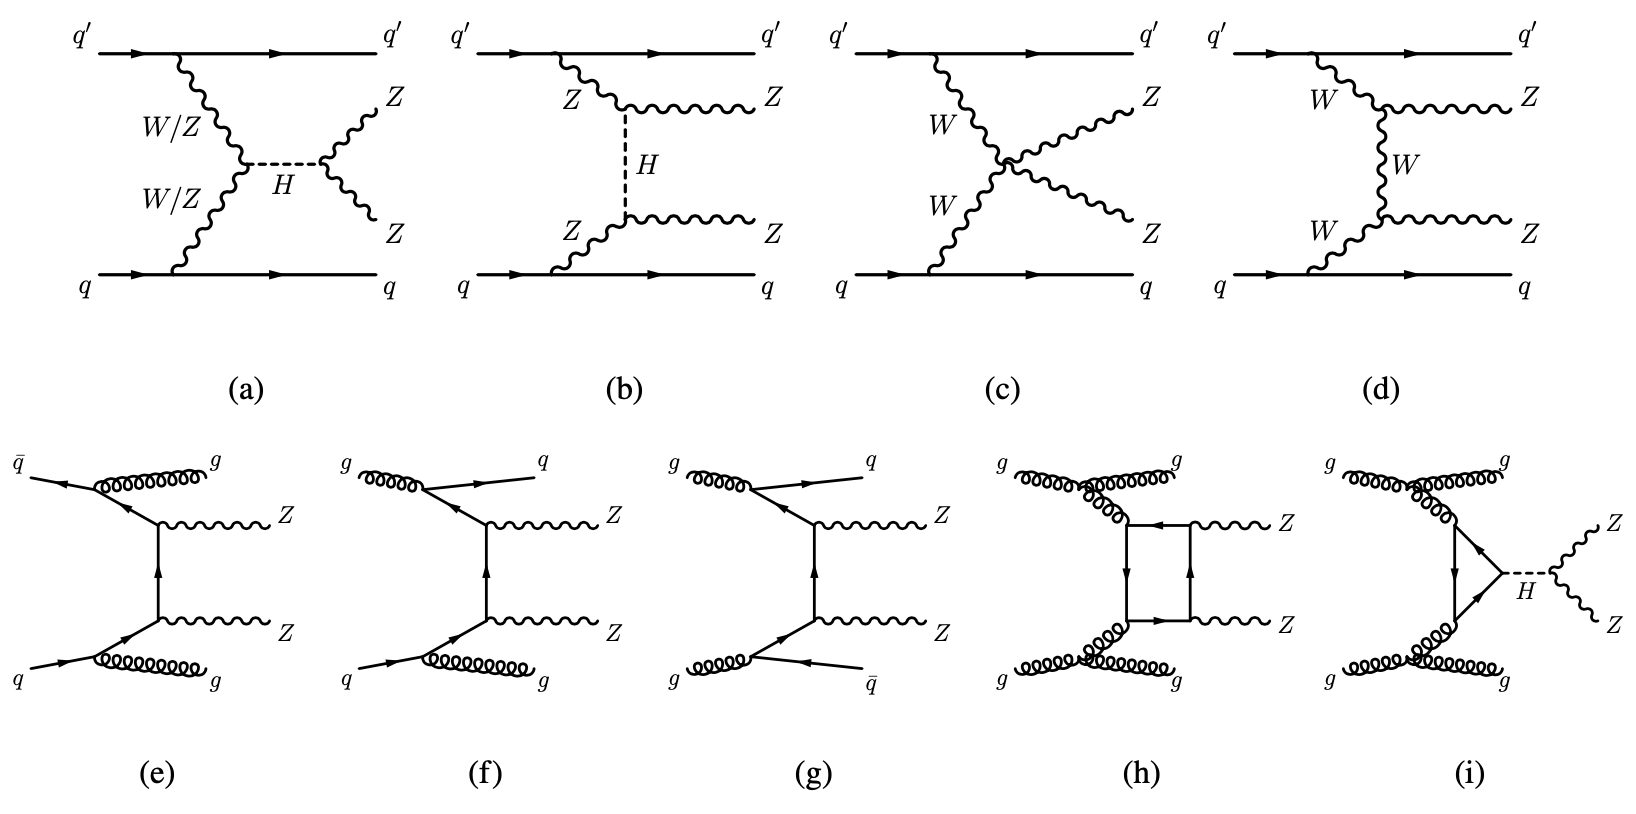
\includegraphics[width=0.95\textwidth]{figures/ch3-LHC-ATLAS/Feynman_vbsZZ.png}
    \caption{Feynman diagrams for $\text{ZZ}jj$ production at the LHC. The diagrams of electroweak $\text{ZZ}jj$ production processes are shown in the top row, and the QCD $\text{ZZ}jj$ production diagrams are shown in the bottom row. }
    \label{fig:zzjj-prod}
\end{figure}

The relevant Feynman diagrams depicting $\text{ZZ}jj$ generation at the LHC are presented in Figure~\ref{fig:zzjj-prod}. For 13~TeV $pp$ collisions within the defined fiducial phase space, the resulting production rate evaluated by \textsc{Sherpa} and \textsc{MadGraph5} is:
$$\sigma^{\text{fid}}_{\text{ZZ}jj \to \ell \ell \nu\nu jj} = 0.94 \pm 0.19\,(\text{QCD scale variation}) \pm 0.01\,(\text{PDF}) \pm 0.02\,(\alpha_s).$$

%\clearpage
%%%%%%%%%%%%%%%%%%%%%%%%%%%%%%%%%%%%%%%%%%%%%%%%%%%%%%%%%%%%%%%%%%%%%%%
%-------------ATLAS----------------
\section{The ATLAS Detector}

Standing as the most massive particle detector ever built for colliding-beam research, the ATLAS detector serves as one of the two primary general-purpose instruments at the LHC~\cite{PERF-2007-01}. Structurally, it adopts a cylindrical configuration, measuring roughly 46~m in length and 25~m in diameter, with an aggregated weight of approximately 7000 tonnes. As illustrated in Figure~\ref{fig:ATLAS-Det-Run2}, the apparatus is organized into a series of concentric sub-detector layers wrapping around the central beamline. Every individual subsystem plays a specific role in capturing the trajectories, momenta, and energies of the diverse particles scattered during proton-proton interactions. 
\begin{figure}[!htbp]
    \centering
    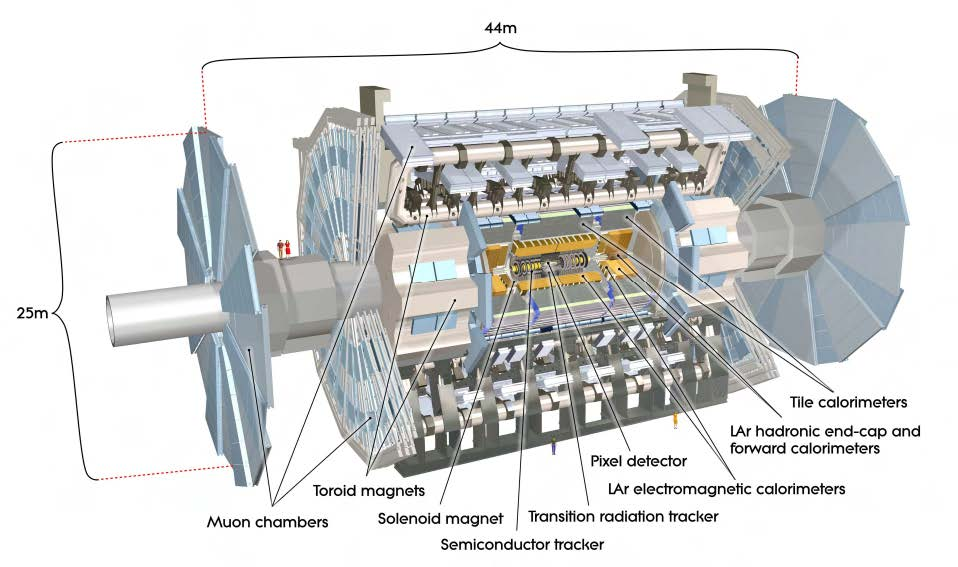
\includegraphics[width=0.95\textwidth]{figures/ch3-LHC-ATLAS/ATLAS_detector_run2.jpg}
    \caption{The ATLAS detector.}
    \label{fig:ATLAS-Det-Run2}
\end{figure}

At its core, the detector is subdivided into the Inner Detector, the intricate calorimeter system, the extensive muon spectrometer, and the powerful magnet system.
The monumental task of designing, assembling, and calibrating this detector spanned a decade and required the collaborative dedication of over 3000 students, engineers, and physicists from the global ATLAS Collaboration. Since the LHC's inaugural run in 2009, this instrument has performed exceptionally well, harvesting pristine collision data continuously through LHC Runs 1, 2, and 3.

To accurately gauge the momenta of charged particles and to precisely reconstruct secondary and primary interaction vertices, the Inner Detector (ID) is utilized. The entirety of the ID volume is enveloped in a $\sim$2~T magnetic field, sustained by a central solenoid. Because this field runs roughly parallel to the $z$-axis, passing charged particles are forced to curve along the $\phi$ direction. By evaluating the geometric curvature of these extracted tracks, physicists can reliably deduce the particle's momentum.

Complementing the ID, the calorimeter system employs specialized sampling techniques to record the energy deposited by both neutral and charged particles. Electromagnetic showers, primarily initiated by photons and electrons, are intercepted and measured by the electromagnetic calorimeter. Conversely, when collision-induced hadrons fragment and cluster into dense particle sprays known as jets, their energy is predominantly absorbed by the hadronic calorimeter. Notably, electromagnetic showers are characteristically more compact and localized, whereas hadronic showers tend to spread extensively across the hadronic calorimeter's volume.

Because muons suffer very little energy loss while traversing the dense materials of the calorimeters and the ID, they act as highly penetrating probes and are eventually registered by the muon spectrometer (MS). Utilizing multiple layers of specialized chambers situated within a massive toroidal magnetic field, the MS secures high-precision muon track coordinates. Depending on the pseudorapidity zone, the integrated bending power of this external magnetic field varies between 1 and 7.5~T$\cdot$m~\cite{PERF-2007-01}. For optimal momentum resolution, track segments identified in the MS are systematically correlated with corresponding tracks originating in the ID.

On the other hand, weakly interacting particles, predominantly neutrinos, slip through the detector entirely undisturbed. Although they leave no direct physical footprint, their existence in an event is mathematically inferred by calculating the vectorial imbalance of all detected transverse momenta. This derived deficit is designated as the missing transverse momentum, $E_{\text{T}}^{\text{miss}}$.

 Table~\ref{tab:detector-performance} details the theoretical design resolutions mapped out for each of the major ATLAS subsystems. Throughout multiple years of proton-proton data-taking at the LHC, the ATLAS detector has reliably fulfilled and often exceeded these ambitious operational targets.

\begin{table}[!htbp]
\centering
\begin{tabular}{lcc}
\hline
\textbf{Detector Component} & \textbf{Required Resolution} & \textbf{$\eta$ Coverage} \\
\hline

Tracking 
& $\sigma_{p_{\text{T}}}/p_{\text{T}} = 0.05\%\,p_{\text{T}} \oplus 1\%$ 
& $|\eta| < 2.5$ \\

Electromagnetic Calorimeter 
& $\sigma_E/E = \frac{10\%}{\sqrt{E}} \oplus 0.7\%$ 
& $|\eta| < 3.2$ \\

Hadronic Calorimeter (barrel and end-cap) 
& $\sigma_E/E = \frac{50\%}{\sqrt{E}} \oplus 3\%$ 
& $|\eta| < 3.2$ \\

Hadronic Calorimeter (forward) 
& $\sigma_E/E = \frac{100\%}{\sqrt{E}} \oplus 10\%$ 
& $3.1 < |\eta| < 4.9$ \\

Muon Spectrometer 
& $\sigma_{p_{\text{T}}}/p_{\text{T}} = 10\%$ at $p_{\text{T}} = 1~\text{TeV}$ 
& $|\eta| < 2.7$ \\

\hline
\end{tabular}
\caption{Performance requirements of major ATLAS detector components.}
\label{tab:detector-performance}
\end{table}


In anticipation of the High-Luminosity LHC (HL-LHC) era slated for 2030, the ATLAS collaboration is rolling out a comprehensive suite of vital upgrades to maximize future discovery potential. These aggressive modifications are essential for shielding the detector's efficiency against the drastic surge in pileup and collision rates projected for the HL-LHC.
%
Chapter~\ref{chap:ATLAS-upgrade} delivers a broad overview of the sweeping ATLAS HL-LHC upgrade agenda. A critical component of this overarching strategy—and a foundational topic of this thesis—is the development and integration of the small-diameter monitored drift tube (sMDT) technology for the muon spectrometer upgrade. An extensive discussion of the sMDT project is provided in Chapters~\ref{chap:sMDT-tube} and~\ref{chap:sMDT-chamber}. 

The subsequent sections of this chapter break down the foundational technologies utilized in the original layout of the ATLAS subdetectors.

%%%%%%%%%%%%%%%%%%%%%%%%%%%%%%%
\subsection{Inner Detector}

Illustrated in Figure~\ref{fig:ID-overview}, the Inner Detector (ID) is primarily composed of three tracking systems: the Transition Radiation Tracker (TRT)~\cite{ATLASTRT2008}, the Semiconductor Tracker (SCT)~\cite{ATLASSCT2008}, and the Pixel detector~\cite{ATLASPixel2008} (further detailed in Figure~\ref{fig:ID-layers}). The fundamental purpose of the ID is to deliver exceptional spatial granularity and precision. This enables the flawless reconstruction of charged-particle trajectories and the accurate determination of impact parameters very close to the collision vertex, an area characterized by extreme particle density.

\begin{figure}[!htbp]
    \centering
    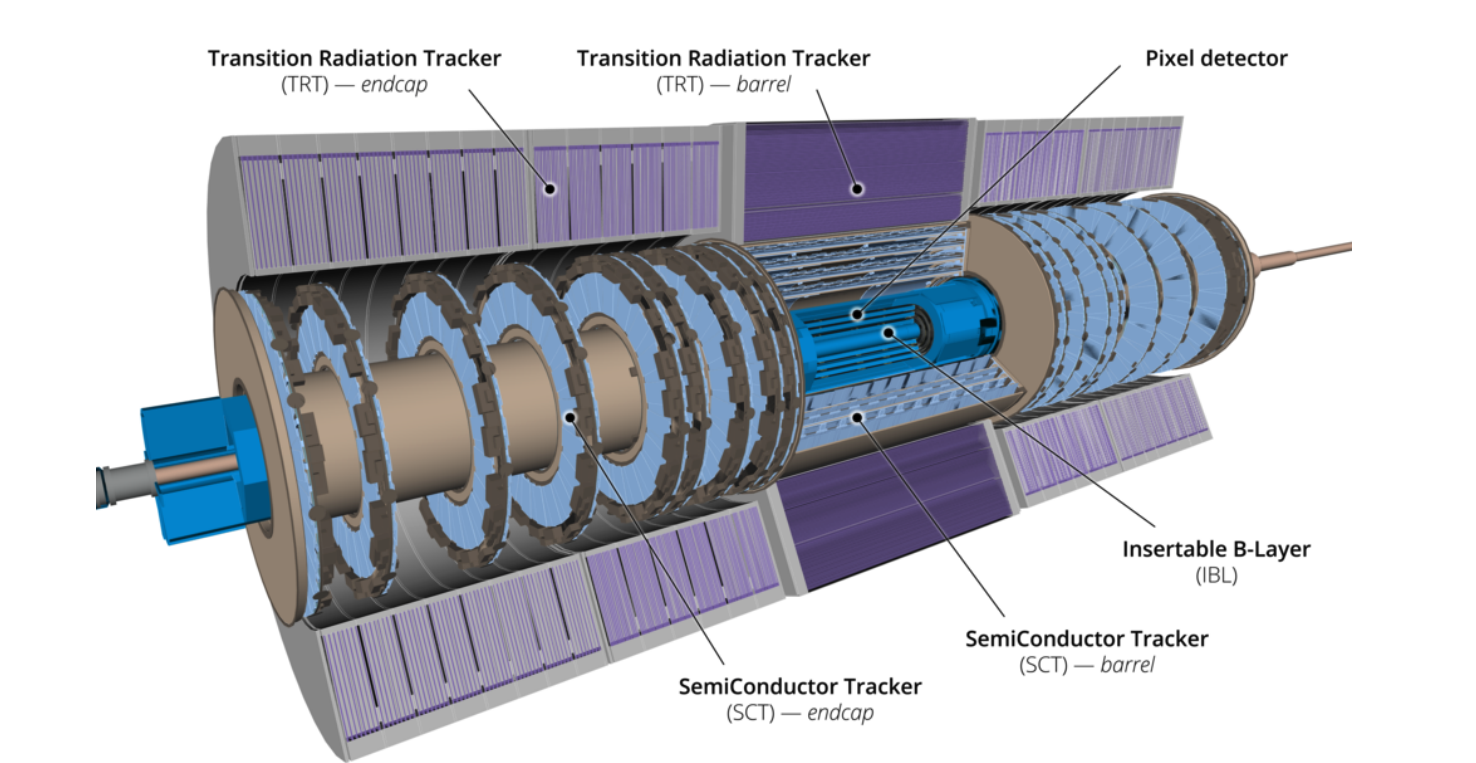
\includegraphics[width=0.95\textwidth]{figures/ch3-LHC-ATLAS/ATLAS_ID_overview.png}
    \caption{The ATLAS Inner Tracker.}
    \label{fig:ID-overview}
\end{figure}

Both the SCT and the Pixel detector leverage advanced silicon-strip and silicon-pixel sensors, respectively, ensuring highly dependable trajectory tracking. As a standard baseline, an escaping charged particle will intersect a minimum of four silicon strip layers and three pixel layers, which provides sufficient data points for rigorous track parameter fitting.

Encasing the silicon layers, the TRT contributes a massive volume of supplemental tracking points, routinely registering up to 36 hits for a single track. By synergizing the diverse datasets from the TRT, SCT, and Pixel modules, the ID achieves uncompromising tracking accuracy and pattern recognition across the entire $\phi$--$z$ geometry.

\begin{figure}[!htbp]
    \centering
    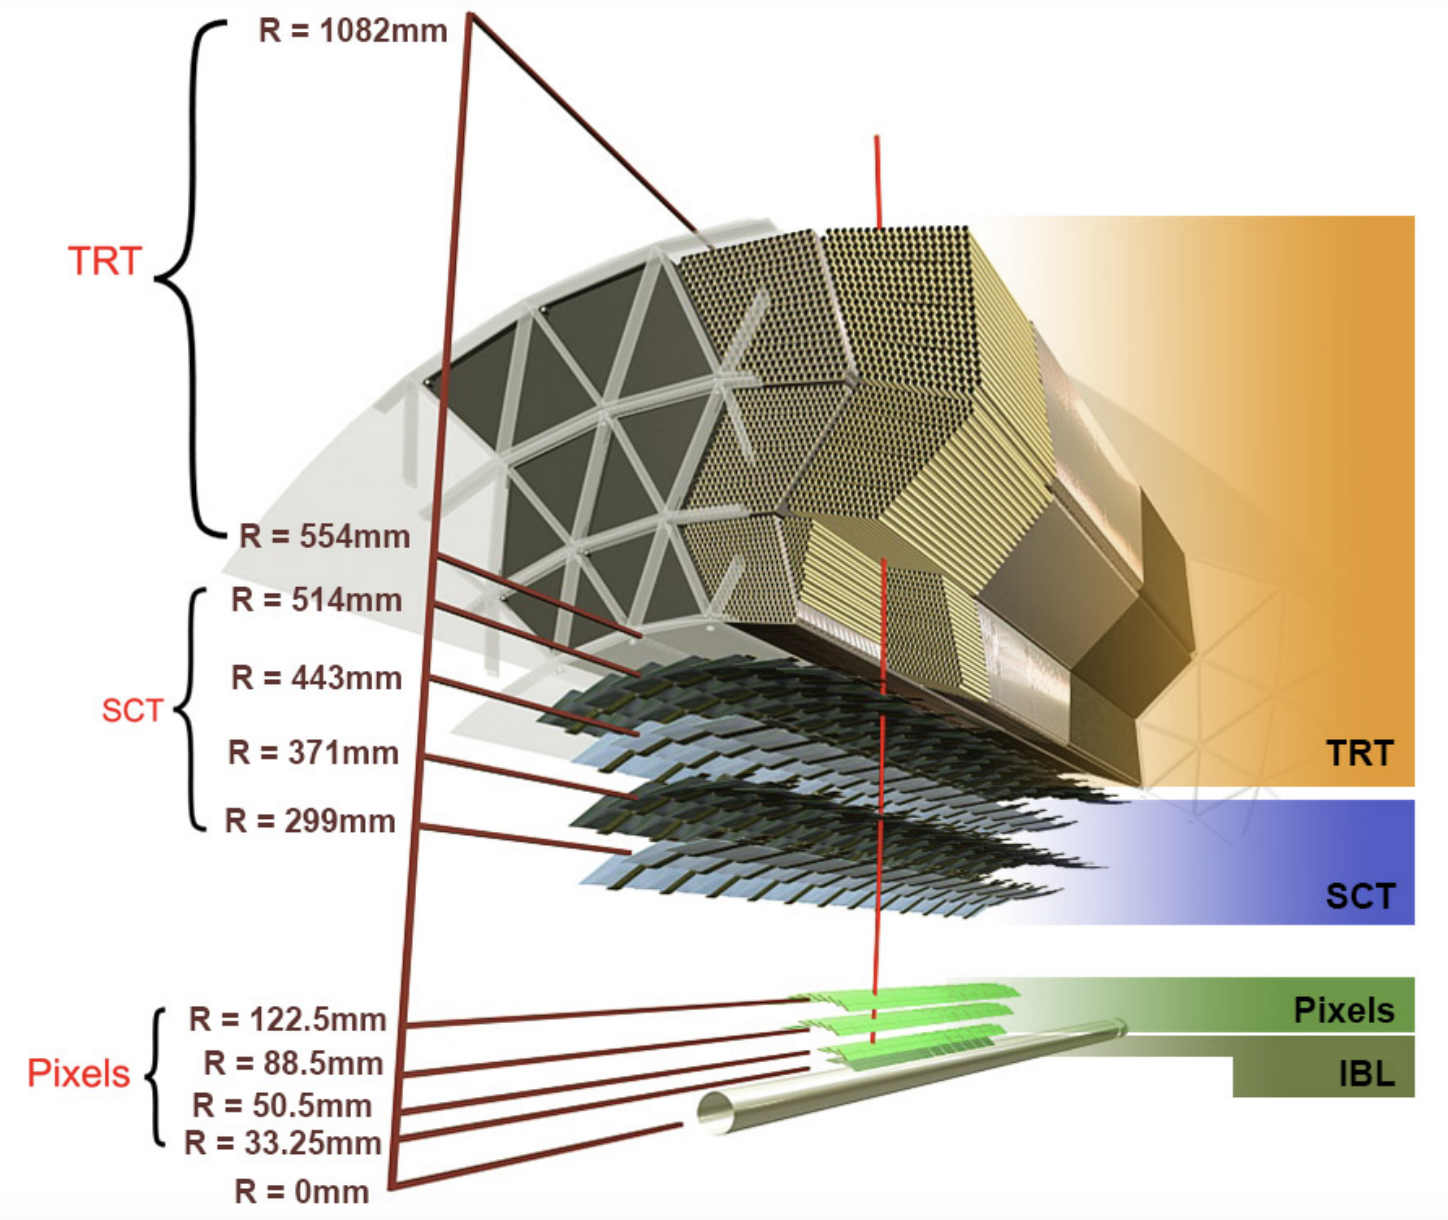
\includegraphics[width=0.35\textwidth]{figures/ch3-LHC-ATLAS/ATLAS_ID_Barrel.png}
    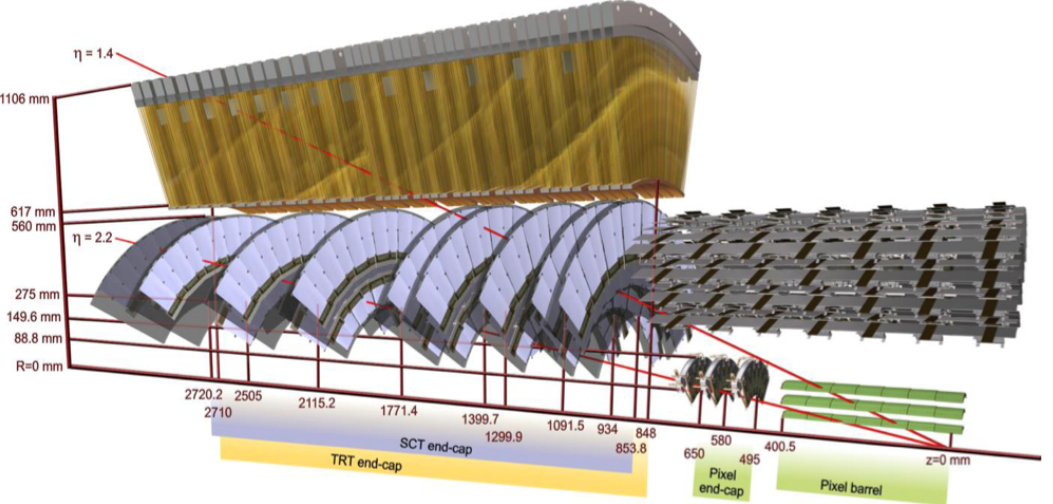
\includegraphics[width=0.63\textwidth]{figures/ch3-LHC-ATLAS/ATLAS_ID_EndCap.png}
    \caption{The 3-dim views of the ID, left panel--barrel, and right panel--end-cap region.}
%    \caption{The ID 3D view in the barrel region \protect\subref{subfig:atlas_id_barrel}~\cite{IDTR-2019-05} and the ID 3D view in the End-Cap region \protect\subref{subfig:atlas_id_endcap}~\cite{Mindur_2016}.}\label{subfig:atlas_id}
    \label{fig:ID-layers}
\end{figure}

Tables~\ref{tab:char_ibl_pixel} and \ref{tab:char_sct_trt} summarize the defining hardware metrics for the various sub-components of the Inner Detector.

\begin{table}[!htbp]
\centering
%\resizebox{0.75\linewidth}{!}{
\begin{tabular}{c|c c}
    \hline\hline
    & \textbf{IBL} & \textbf{Pixel} \\
    \hline
    \textbf{Element Size}  &  $50~\mu\text{m} \times 250~\mu\text{m}$ &  $50~\mu\text{m} \times 400~\mu\text{m}$ \\
    \textbf{Intrinsic Resolution in \boldmath $r-\phi$ ($\mu$m)}  & 10  & 10  \\
    \textbf{Intrinsic Resolution in \boldmath $z$} ($\mu$m) & 60  &  115 \\
    \textbf{Barrel Layer Radii (mm)}  & 33.25  &  50.5, 88.5, 122.5 \\
    \textbf{Disk Layer \boldmath $|z|$ (mm)}  &   &   495, 580, 650 \\
    \hline\hline
\end{tabular}
\caption{Main Characteristics of the IBL and Pixel Detectors.}
\label{tab:char_ibl_pixel}
\end{table}

\begin{table}[!htbp]
\centering
%\resizebox{0.75\linewidth}{!}{
\begin{tabular}{c|c c}
\hline\hline
 & \textbf{SCT} & \textbf{TRT} \\
\hline
\textbf{Element Size}  &  $80~\mu\text{m}$ & 4 mm \\
\textbf{Intrinsic Resolution in \boldmath $r-\phi$ ($\mu$m)}  & 17  & 130 \\
\textbf{Barrel Layer Radii (mm)}  & 299, 371, 443, 514 & $554-1082$ \\
\textbf{Disk Layer \boldmath $|z|$ (mm)} &  $839-2735$ & $848 - 2710$ \\
\hline\hline
\end{tabular}
\caption{Main Characteristics of the SCT and TRT detector.}
\label{tab:char_sct_trt}
\end{table}
\FloatBarrier

%%%%%%%%%%%%%%%%%%%%%%%
\subsection{The Calorimeters}

Comprising multiple subdetectors based on diverse technologies, the ATLAS calorimeter system~\cite{ATLAS-TDR-04,ATLAS-TDR-05} (displayed in Figure~\ref{fig:atlas_calo}) is specifically engineered to meet stringent physics demands while withstanding the LHC's intense radiation environment. Through these interconnected systems, the ATLAS framework guarantees near-total solid-angle visibility for tracking particles up to a pseudorapidity boundary of $|\eta| < 4.9$.

\begin{figure}[!htbp]
\centering
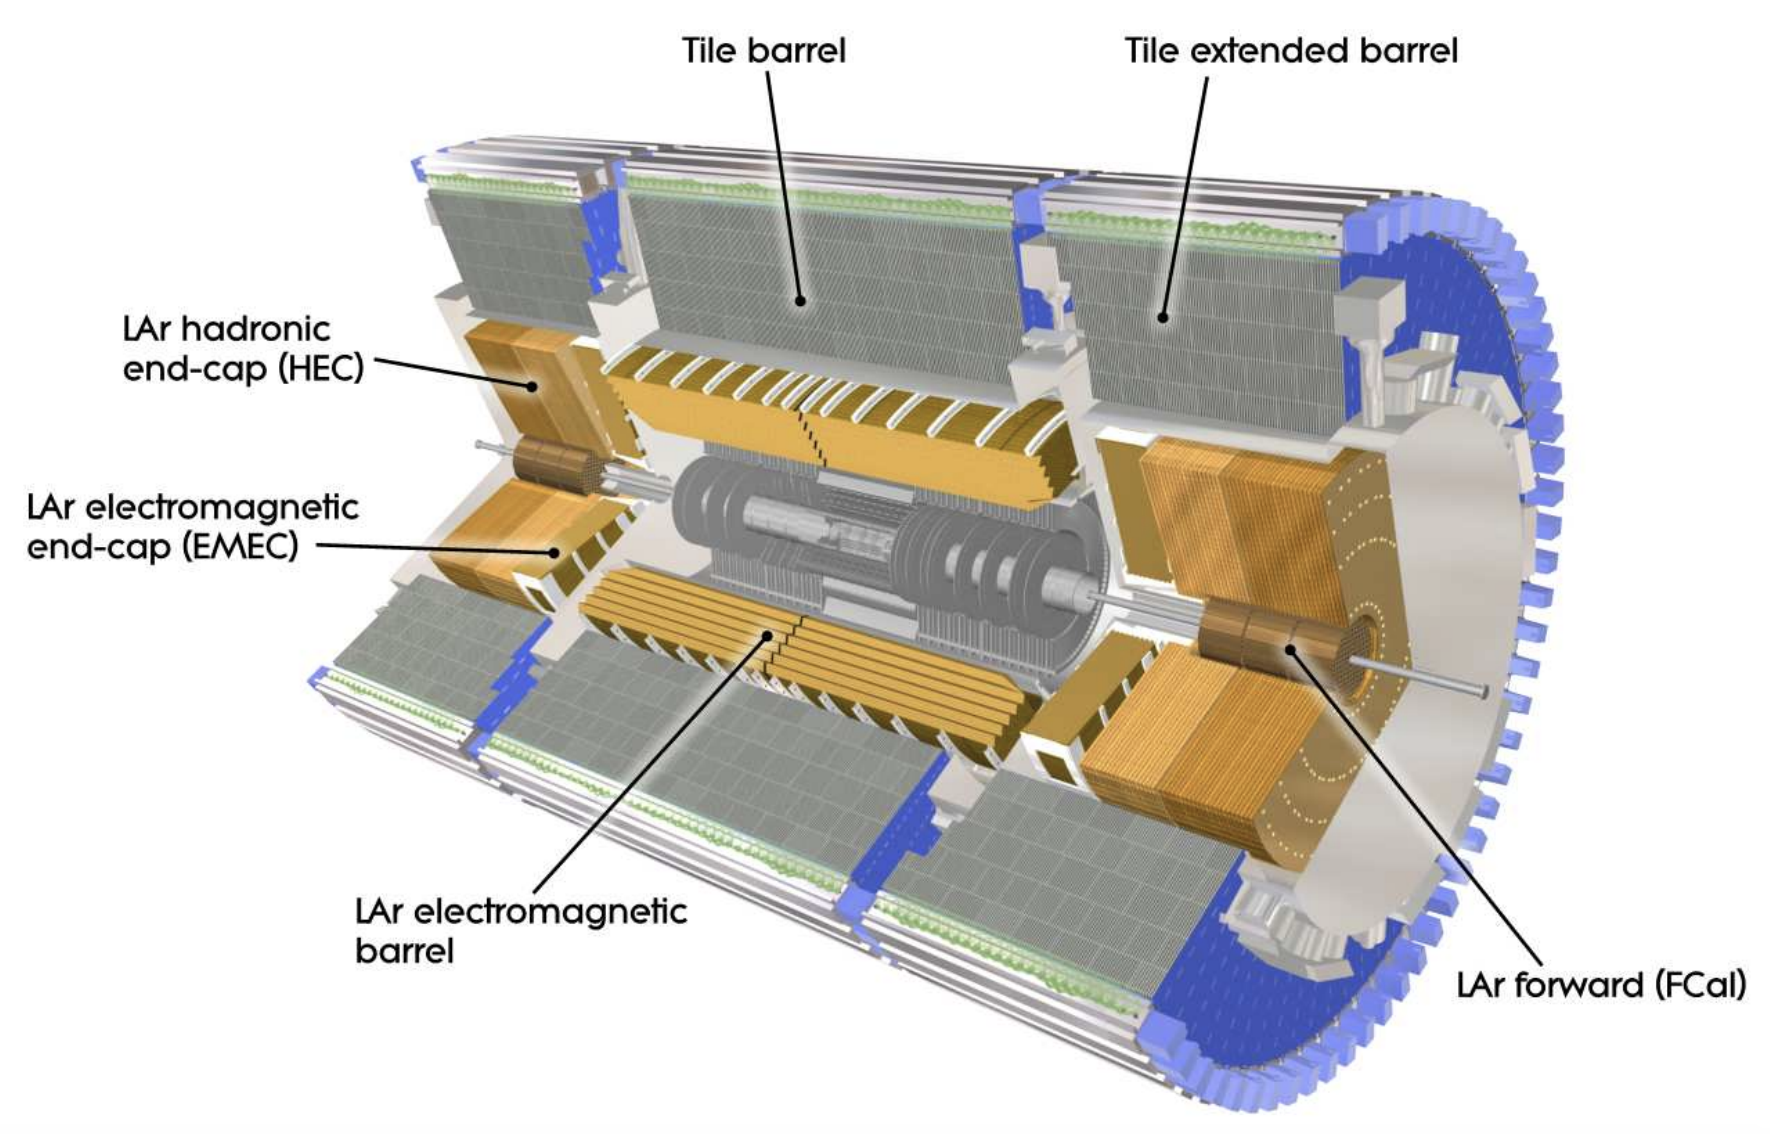
\includegraphics[width=0.8\textwidth]{figures/ch3-LHC-ATLAS/ATLAS_Calorimeters.png}
\caption{A cut-away view of the ATLAS calorimeters~\cite{PERF-2007-01}.}
\label{fig:atlas_calo}
\end{figure}

For the region overlapping with the Inner Detector's acceptance, the electromagnetic (EM) calorimeter provides an exceptionally fine spatial resolution, perfect for accurately charting photon and electron kinematics. The hadronic calorimeters, however, rely on a coarser segmentation strategy; this is entirely adequate for profiling the broader topologies of hadronic jets and for determining the missing transverse energy ($E_{\text{T}}^{\text{miss}}$). 

\textbf{The EM calorimeter} boasts a formidable depth, reaching over 24 radiation lengths ($X_0$) in the end-cap sections and exceeding 22 $X_0$ throughout the barrel. When fused with the shielding of the hadronic calorimeters, this substantial density ensures that nearly all hadronic and electromagnetic showers are trapped completely within the calorimeter boundaries. This containment strictly limits any erroneous energy spillover into the outer muon spectrometer.

Fundamentally, the EM calorimeter operates as a sampling device utilizing liquid-argon (LAr) as the active material, interspersed with lead absorber plates and distinctively ``accordion-shaped'' Kapton electrodes~\cite{ATLAS-TDR-04}. This innovative accordion geometry guarantees an uninterrupted azimuthal ($\phi$) symmetry, eliminating dead-zone cracks and promoting rapid, homogeneous signal readouts.

Spatially, the EM barrel (EMB) component handles the pseudorapidity interval $|\eta| < 1.475$, while the two EM end-cap (EMEC) sections cover the $1.375 < |\eta| < 3.2$ domain. Both the end-cap and barrel segments reside within three isolated LAr-filled cryostats. For the core region ($|\eta| < 2.5$), the system is sliced into three longitudinal layers:

\begin{itemize}

\item \textbf{First layer (strip layer):}  
This front-line layer spans $1.5 < |\eta| < 2.4$ and $|\eta| < 1.4$, presenting a thickness of approximately $4.4\,X_0$.  
Its extreme granularity in $\Delta\eta \times \Delta\phi$ (roughly $0.003 \times 0.1$ in the EMB) is its defining feature.  
Because of this ultra-fine segmentation, physicists can successfully distinguish standalone photon showers from overlapping photon pairs caused by neutral pion decays (e.g., $\pi^0 \rightarrow \gamma\gamma$).

\item \textbf{Second layer (L2):}  
Functioning as the primary energy sink, this layer captures the bulk of the shower energy generated by incoming photons and electrons.  
It extends to a depth of roughly $17\,X_0$ and features a spatial resolution of $0.025 \times 0.025$ in the $\Delta\eta \times \Delta\phi$ plane.

\item \textbf{Third layer (L3):}  
Characterized by a $0.05 \times 0.025$ granularity in $\Delta\eta \times \Delta\phi$ and an approximate depth of $2\,X_0$.  
The main function of L3 is tracking the tail-end of showers to correct for any minor energy leakage exiting the rear of the EM calorimeter.

\item \textbf{Presampler layer (PS):}  
Situated directly in front of the calorimeter for regions up to $|\eta| < 1.8$, this slim detector layer plays a crucial role.  
It is deployed to measure and offset the energy that electrons or photons might have prematurely deposited in the structural materials upstream.  
The PS operates with a granularity of $0.025 \times 0.1$ in $\Delta\eta \times \Delta\phi$.

\item \textbf{Transition region:}  
The boundary gap separating the end-cap and barrel calorimeters ($1.37 < |\eta| < 1.52$) is populated with a considerable volume of inactive infrastructure. Consequently, energy resolution in this specific transition zone is inherently degraded.

\end{itemize}
\begin{table}[!htbp]
    \small
    \centering
    \begin{tabular}{c|c|c|c|c}
        \hline\hline
        \textbf{EM Calorimeter} & \multicolumn{2}{c|}{\textbf{Barrel}} &\multicolumn{2}{c}{\textbf{End-Cap}} \\
        \hline
         & \textbf{\# of Layers} & \textbf{$|\eta|$ coverage} & \textbf{\# of Layers} & \textbf{$|\eta|$ coverage} \\
         \hline
         Presampler & 1 & $|\eta|<1.52$ & 1 & $1.5<|\eta|<1.8$ \\
         \hline
         \multirow{3}{*}{Calorimeter} & 3 & $|\eta|<1.35$ & 2 & $1.375<|\eta|<1.5$ \\
         & 2 & $1.35<|\eta|<1.475$ & 3 & $1.5<|\eta|<2.5$ \\
         & & & 2 & $2.5<|\eta|<3.2$ \\
        \hline\hline
    \end{tabular}
    \caption{Some important parameters of the EM calorimeter.}
    \label{tab:EMCal_parameters}
\end{table}

%%%%%%%%%%%%%%%%%
\textbf{The hadronic calorimeters (HCAL)} framework merges three distinct subsystems. Their collective goal is to gauge hadronic energy and reinforce the electromagnetic calorimeter's data, which is crucial for precise jet clustering and missing transverse energy derivation.

\begin{itemize}

\item \textbf{Tile Calorimeter:}

Positioned immediately outward from the EM calorimeter, the Tile Calorimeter~\cite{ATLAS-TDR-05} acts as the primary central hadronic detector for the ATLAS suite. Operating as a sampling calorimeter, it incorporates scintillating plastic tiles for the active readout and thick steel plates for the absorber matrix.

Coverage for the central barrel section extends to $|\eta| < 1.0$, whereas adjacent extended barrel modules push this reach out to $0.8 < |\eta| < 1.7$. Radially, the device occupies the space between 2.28~m and 4.25~m away from the beam axis.

Internally, it is stratified into three distinct radial layers. In the central barrel, these layers represent depths of roughly 1.5, 4.1, and 1.8 interaction lengths ($\lambda$); in the extended barrels, the depths shift to 1.5, 2.6, and 3.3 $\lambda$. Photons emitted by the scintillating tiles are routed via wavelength-shifting fibers to dual independent photomultiplier tubes (PMTs) situated on either side, establishing a robust, redundant readout architecture.

\item \textbf{LAr Hadronic End-Cap Calorimeter (HEC):}

Installed directly behind the EM end-cap calorimeters, the HEC~\cite{ATLAS-TDR-04} assumes responsibility for capturing hadronic energy signatures across the forward/end-cap zones. Every end-cap module is constructed from two standalone wheels.

Similar to the EM system, the HEC is a liquid-argon-based sampling calorimeter, though it substitutes lead for copper plates as its heavy absorber. Geometrically, wedge-shaped modules are interlocked to assemble the complete circular wheels.

Each of these end-caps is longitudinally partitioned into four layers. The copper absorbers boast an outer radius of nearly 2.03~m and an inner opening radius of about 0.475~m. Approaching the junction between the forward calorimeter (FCal) and the HEC, this inner radius shrinks to roughly 0.372~m.

To prevent any dangerous gaps in detection efficiency or material density, the HEC is designed to overlap seamlessly with the Tile calorimeter (covering up to $|\eta| \approx 1.5$) and the forward calorimeter (extending out to $|\eta| \approx 3.2$).

\item \textbf{LAr Forward Calorimeter (FCal):}

Housed directly within the end-cap cryostat assemblies, the FCal~\cite{ATLAS-TDR-04} manages calorimetric data acquisition in the extreme forward geometries. Because it sits incredibly close to the beamline, it is heavily reinforced to survive an environment plagued by astronomical particle fluxes and severe radiation.

Structurally, the FCal extends to an overall depth of roughly $10\,\lambda$ and is modularized into three segments. The innermost module relies on copper absorbers to specialize in electromagnetic tracking. Conversely, the second and third modules utilize tungsten to optimize the containment and measurement of intense hadronic showers.

This detector features a unique metal matrix design utilizing parallel, concentric tubes and rods aligned with the beam axis to act as electrodes. The microscopic void between the rods and the tubes is flooded with liquid argon, which serves as the active medium for capturing the ionization signals.

\end{itemize}


\begin{table}[!htbp]
    \small
    \centering
    \begin{tabular}{c|c|c|c}
        \hline\hline
         & \textbf{\# of Layers} & \textbf{$|\eta|$ coverage} & \textbf{Readout channels} \\
        \hline
        \textbf{Tile calorimeter (Barrel)} & 3 & $|\eta|<1.0$ & 5760 \\
        \textbf{Tile calorimeter (Extended Barrel)} & 3 & $0.8<|\eta|<1.7$ & 4092 (both sides) \\
        \textbf{LAr hadronic end-cap} & 4 & $1.5<|\eta|<3.2$ & 5632 (both sides) \\
        \textbf{LAr forward calorimeter} & 3 & $3.1<|\eta|<4.9$ & 3524 (both sides) \\
        \hline\hline
    \end{tabular}
    \caption{Some important parameters of the hadronic calorimeter.}
    \label{tab:HadCal_parameters}
\end{table}

The ultimate energy resolution capability of the calorimeters is constrained by an array of physical fluctuations. These include inherent shower development anomalies, photoelectron statistical variations, energy leakage out of the detector volume, and hardware-induced noise (like light attenuation issues, structural non-uniformities, and basic electronic interference).
%
Because the ATLAS calorimeters utilize a alternating sampling strategy (absorber vs. active layer), sampling fluctuations introduce another layer of variance into the final energy measurement.
%
Consequently, physicists generally model the energy resolution of a calorimeter using the formula:
\begin{equation}\label{eq:energy-resolution}
    \frac{\sigma_E}{E} = \frac{a}{\sqrt{E}} \oplus \frac{b}{E} \oplus c ,
\end{equation}
where the $\oplus$ symbol indicates that the terms are added in quadrature.

Within Equation~\eqref{eq:energy-resolution}, the first variable represents the \textit{stochastic term}, driven primarily by statistical anomalies inherent in the sampling mechanism and shower expansion. Next is the \textit{noise term}, which encapsulates the environmental and hardware interference, such as pile-up noise and baseline electronic static. Finally, the \textit{constant term} corrects for macroscopic hardware flaws, such as slight detector non-linearities, imperfect calibrations between adjacent cells, and structural inhomogeneities.
%
Because the stochastic term is a fundamental physical limitation of the calorimetric method, it is virtually impossible to eliminate. Meanwhile, the noise term exerts its strongest influence on low-energy particle readings, while the constant term dictates the resolution ceiling for highly energetic particles.
%
For hadronic calorimeters specifically, the energy deposited by hadronic showers easily dwarfs the baseline electronic static, allowing physicists to routinely safely ignore the noise term ($b/E$).
%
The established energy resolution benchmarks for both the hadronic and electromagnetic calorimeters have been documented previously in Table~\ref{tab:detector-performance}.

%%%%%%%%%%%%%%%%%%%%%%%%%%%%%%%%%%%
\subsection{Muon Spectrometer}
\label{chap:MS}

Positioned as the outermost shell of the ATLAS apparatus, the Muon Spectrometer (MS)~\cite{ATLAS-TDR-10,muonRecoPerf21} (illustrated in Figure~\ref{fig:ATLAS_MS_run2}) is designed to capture muons, which effortlessly pass through the inner detector and calorimeter layers. To achieve a seamless blend of high-precision tracking and rapid trigger capabilities, the MS incorporates a mixture of diverse detector technologies. 
\begin{figure}[!htbp]
    \centering
    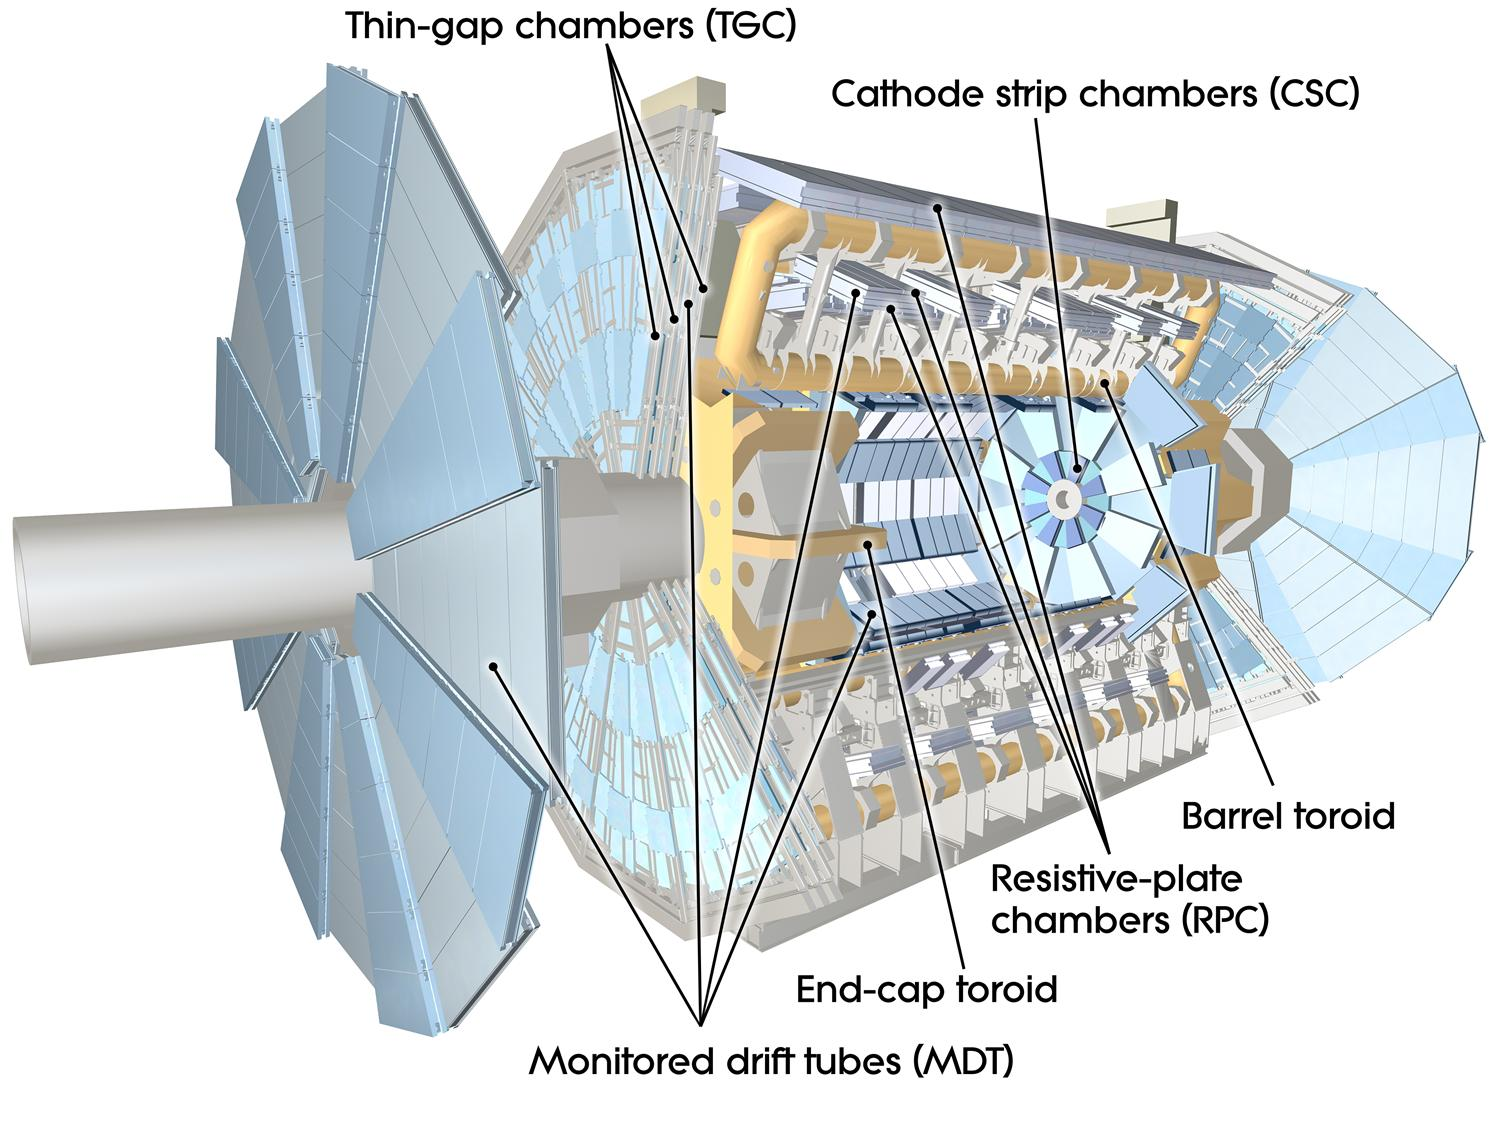
\includegraphics[width=0.75\textwidth]{figures/ch3-LHC-ATLAS/ATLAS-MS.jpg}
    \caption{Cut-away view of the Run~2 configuration of the ATLAS detector indicating the locations of the major detector sub-systems~\cite{detector_Aad_2024}.}
    \label{fig:ATLAS_MS_run2}
\end{figure}
\begin{figure}[!htbp]
    \centering
    \subfloat[]{
    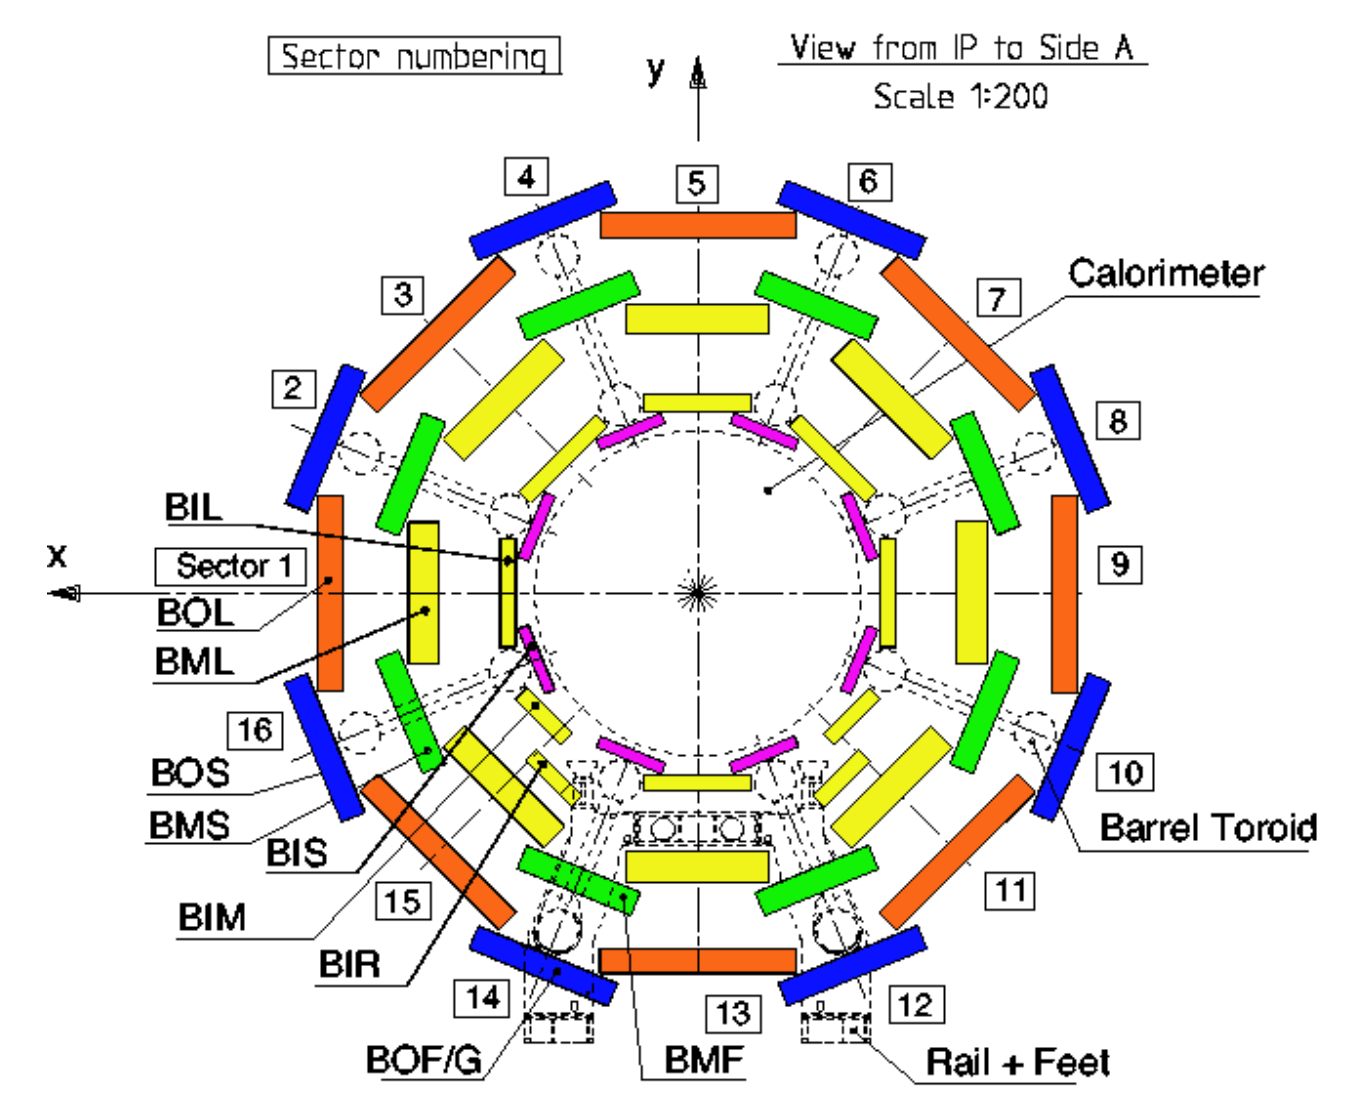
\includegraphics[width=0.41\textwidth]{figures/ch3-LHC-ATLAS/ATLAS-MS-XY.png}
    }
    \subfloat[]{
    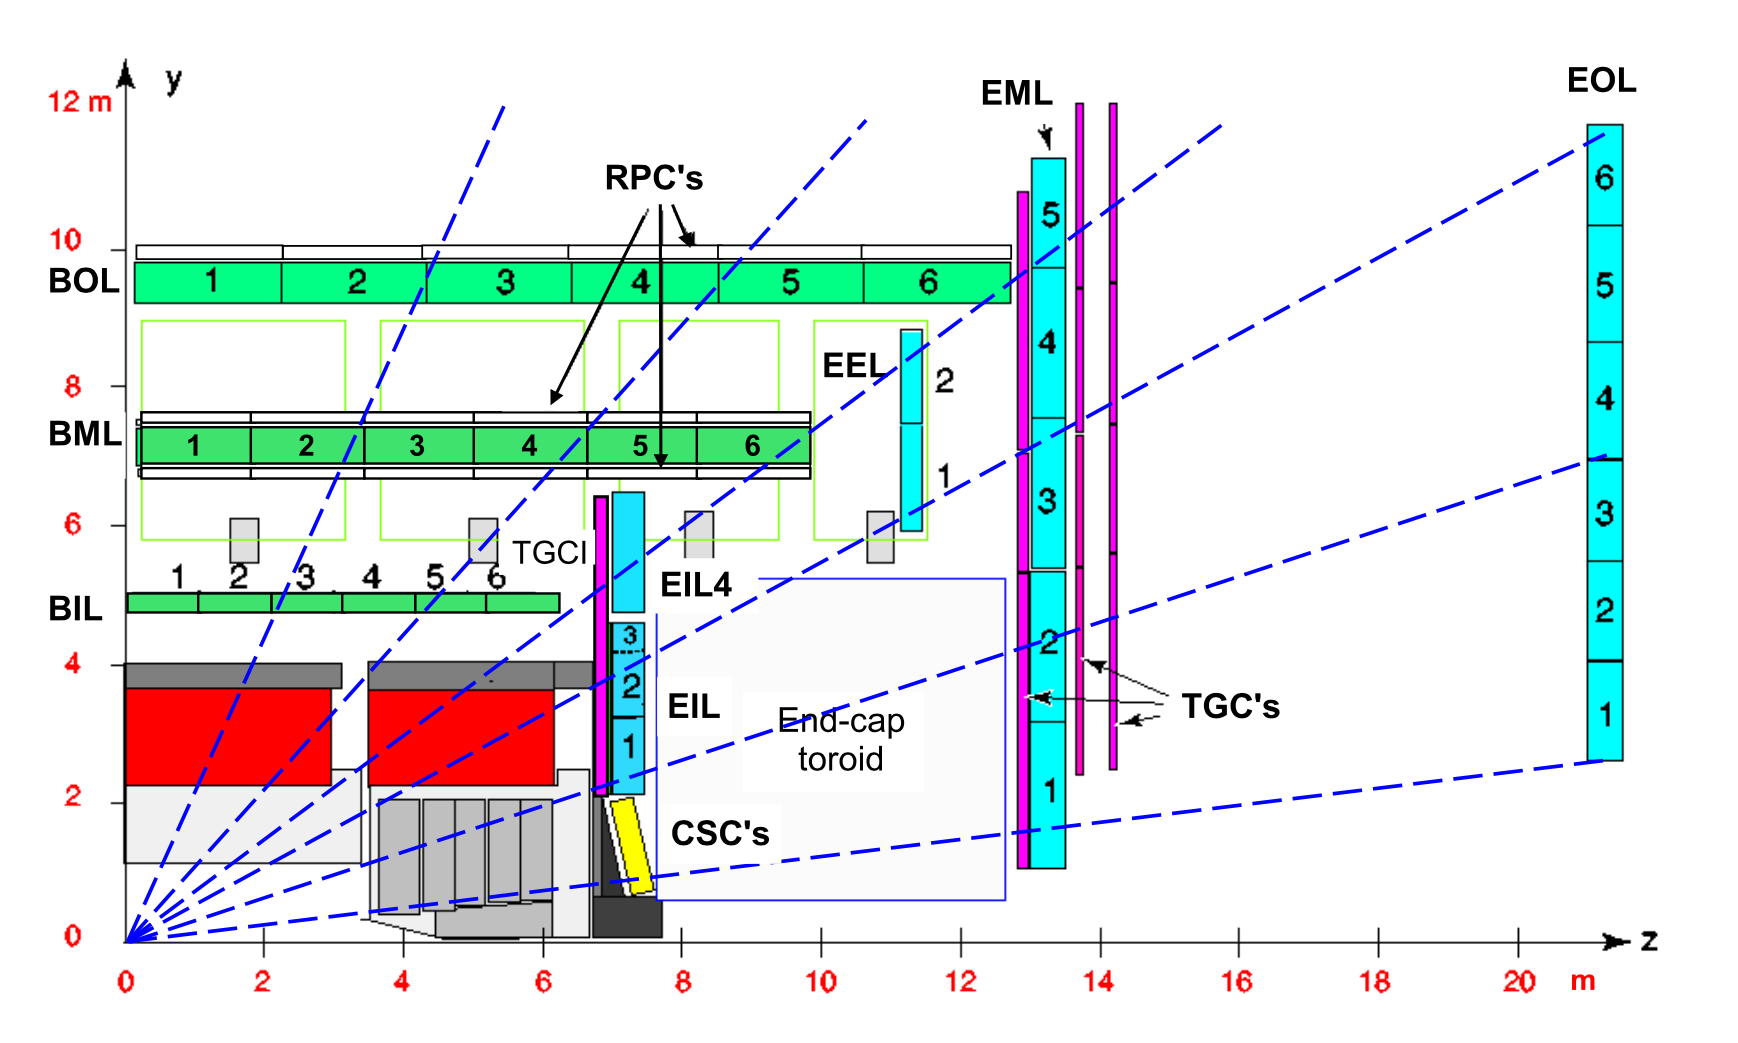
\includegraphics[width=0.575\textwidth]{figures/ch3-LHC-ATLAS/ATLAS-MS-RZ.png}
    }
    \caption{The ATLAS MS Barrel (a) and End-cap (b), layout for Run~1 and Run~2 operations.}
    \label{fig:MS-layout}
\end{figure}

The overarching layout of the MS across both the End-cap and Barrel regions is mapped in Figure~\ref{fig:MS-layout}.
Gigantic air-core superconducting toroidal magnets are employed to curve the muon trajectories. For central tracks ($|\eta|<1.4$), the barrel toroid takes charge of the bending. In the outer fringes ($1.6<|\eta|<2.7$), the end-cap toroid magnets generate the required force. In the transitional overlap slice ($1.4<|\eta|<1.6$), the magnetic fields from both toroid systems intersect and contribute jointly. Because the magnetic field vectors are aligned almost perfectly perpendicular to the paths of the outward-bound muons, the magnet system excels at curving the tracks while minimizing resolution errors caused by multiple scattering. This orchestrated track deflection is subsequently mapped in the $r$-$z$ plane.

Throughout the data-taking eras of Run~1 and Run~2, the MS framework merged four distinct detector types: Cathode Strip Chambers (CSC) and Monitored Drift Tubes (MDT) were tasked with precision coordinate tracking, whereas Thin Gap Chambers (TGC) and Resistive Plate Chambers (RPC) handled the fast muon triggering. To ensure complete coverage, the MS deploys three TGC stations in the end-caps and three RPC stations in the barrel. The MDT arrays handle the bulk of the precision tracking across the vast majority of the MS volume. Conversely, CSC modules are reserved exclusively for the innermost ring of the end-cap zones, an area defined by exceptionally high particle flux rates. A breakdown of these distinct muon technologies follows below.

\noindent\textbf{Monitored Drift Tube (MDT) detectors}   \\
Detailed in Figure~\ref{fig:MDT_struct}, MDT chambers are built from pressurized aluminum tubes sporting an internal diameter of 29.7 mm. These tubes are injected with a gas blend of 7\% CO$_2$ and 93\% Ar, tightly pressurized to 3~bar. As a charged particle breaches the tube wall, it triggers gas ionization. The freed electrons immediately drift inward toward a 50~$\mu$m tungsten–rhenium core wire, which is constantly electrified at a working voltage of 3080~V.
\begin{figure}[!htbp]
    \centering
    \subfloat[]{
        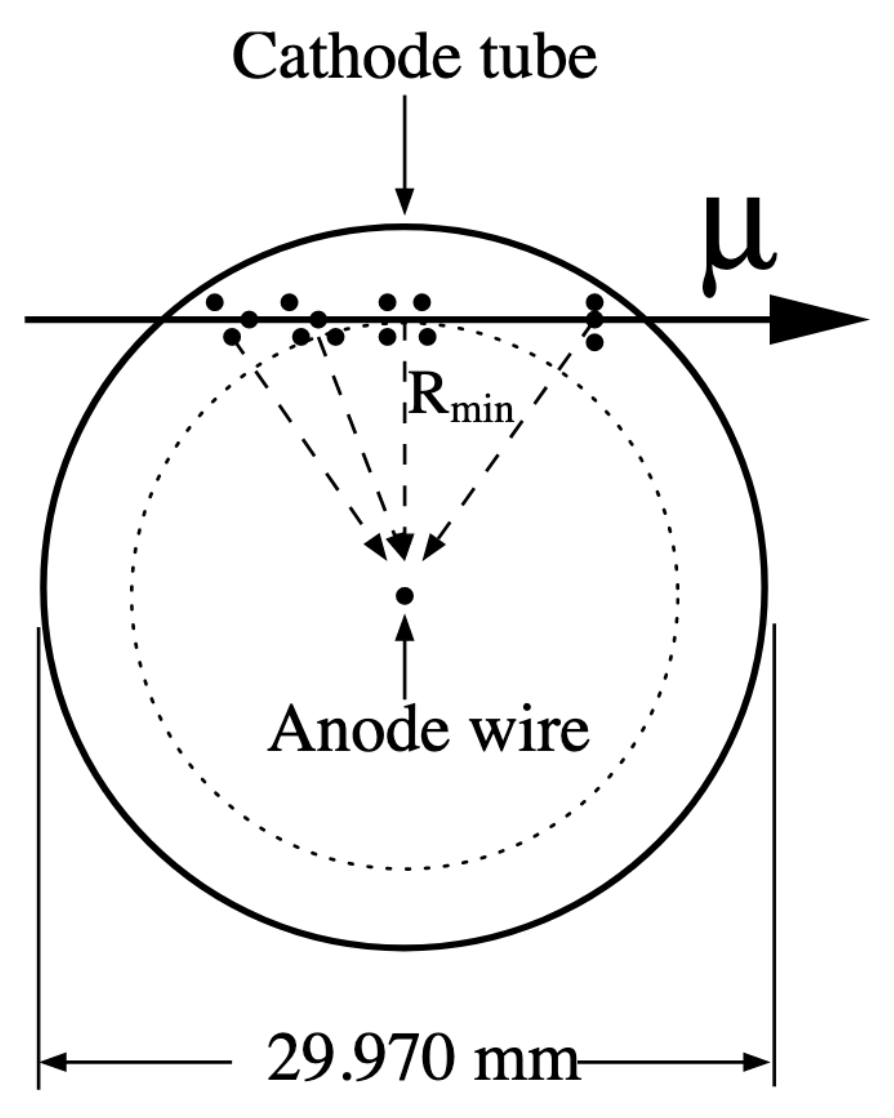
\includegraphics[width=0.3\textwidth]{figures/ch3-LHC-ATLAS/MDT_Tube_diagram.png}
        \label{subfig:mdt_tube_diag}
    }
    \qquad
    \subfloat[]{
        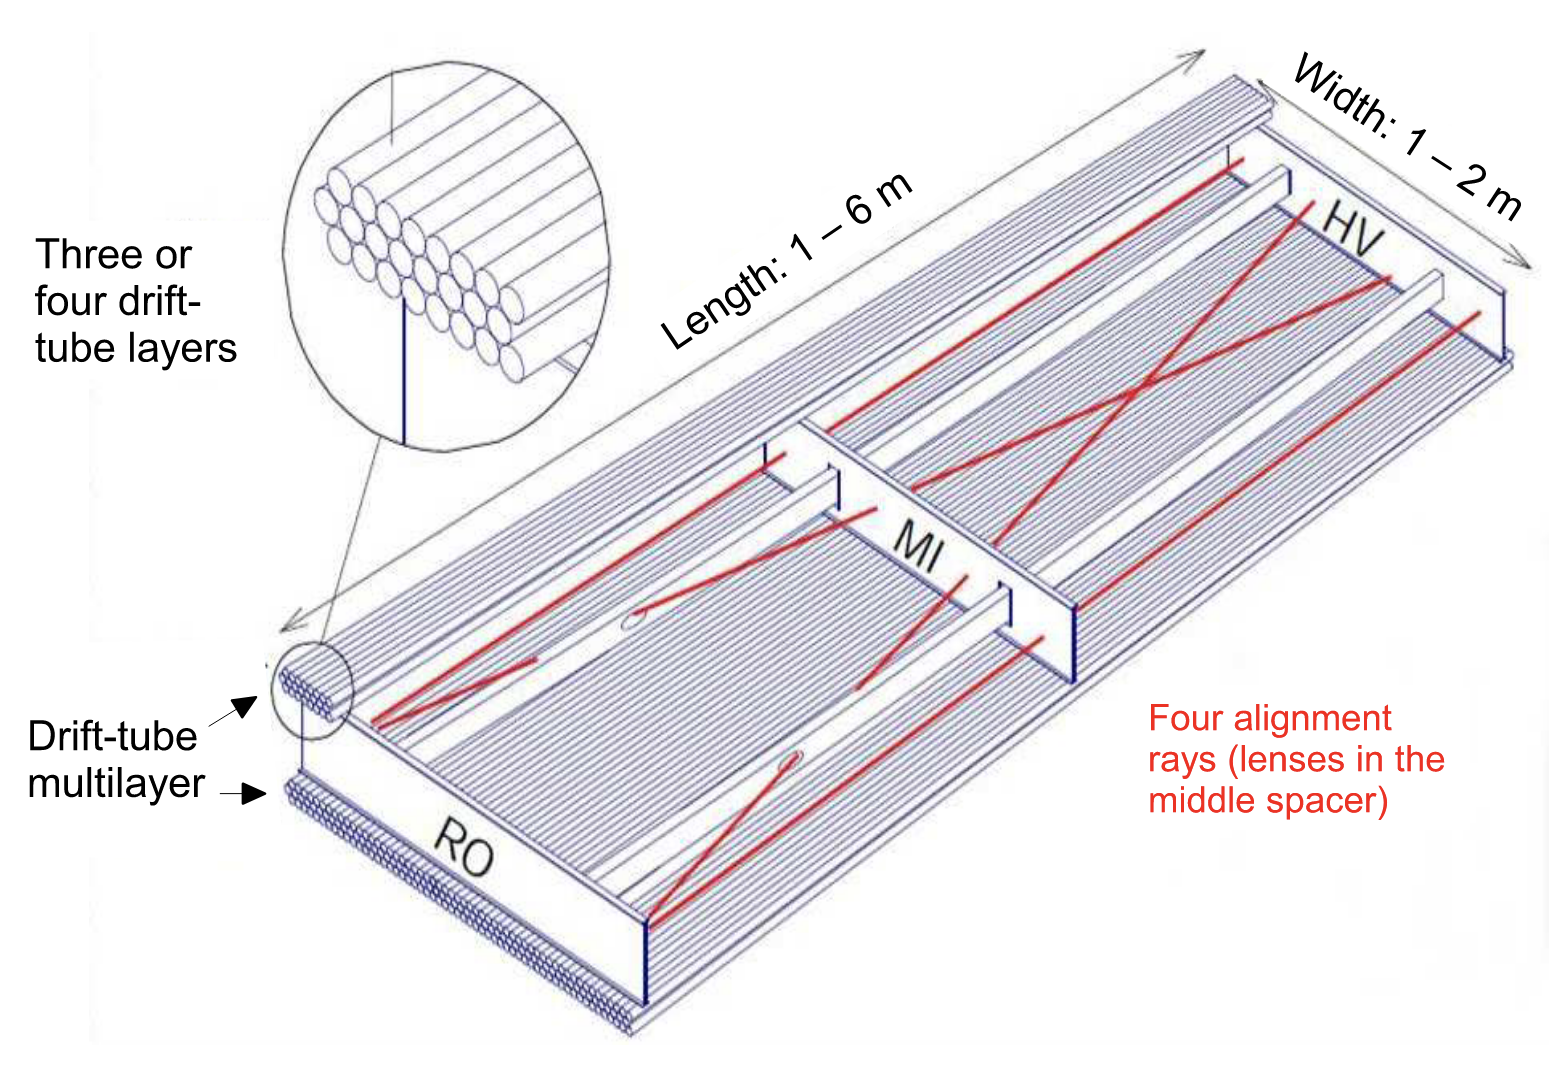
\includegraphics[width=0.6\textwidth]{figures/ch3-LHC-ATLAS/MDT_MechStruct.png}
        \label{subfig:mdt_mechstruct}
    }
    \caption{(a) Cross-sectional view of an MDT tube showing ionization clusters along the particle track~\cite{YArai_2008}; (b) mechanical structure of an MDT chamber~\cite{PERF-2007-01}. Each chamber consists of two multilayer groups, each with three (or four) layers, separated by a support structure.}
    \label{fig:MDT_struct}
\end{figure}
%
From a structural standpoint, an individual MDT chamber is formed by two multilayer groups rigidly held apart by a specialized mechanical spacer. To boost pattern recognition efficiency near the collision center, the innermost multilayer block utilizes four stacked tube layers, whereas the middle and outer blocks rely on three layers (see Figure~\ref{fig:MDT_struct}). This specific MDT architecture is prized for delivering remarkable operational stability and mechanical rigidity. Furthermore, because the internal electric field is strictly radial, the impact of a particle's entry angle on the ultimate spatial resolution is negligible. In practice, individual tubes routinely achieve their design resolution target of roughly 80~$\mu$m~\cite{PERF-2007-01}.

\begin{table}[!htbp]
    \centering
    \begin{tabular}{l|c}
        \hline\hline
        \textbf{MDT Parameter} & \textbf{Value} \\
        \hline
        Gas mixture & Ar/CO$_2$ (93\%/7\%) \\
        Operating voltage & 3080 V \\
        Wire material & W/Re (97\%/3\%); 3\% gold plating \\
        Gas pressure & 3 mbar (absolute) \\
        Gas gain & $2\times10^4$ \\
        Maximum drift time & $\sim 750$ ns \\
        Average tube resolution & $\sim 80$ $\mu$m\\
        \hline\hline
    \end{tabular}
    \caption{Summary of important parameters of the Monitored Drift Tube chamber.}
    \label{tab:summary_MDT}
\end{table}

\vspace{0.3cm}
\noindent \textbf{Cathode Strip Chambers (CSCs)} \\
Functioning as specialized multiwire proportional chambers, CSCs leverage an array of radially aligned anode wires held at an approximate voltage of 1900~V. The active ionizing medium filling the chambers is an 80\%/20\% mix of Ar/CO$_2$. 
\begin{figure}[!htbp]
    \centering 
    \subfloat[]{
    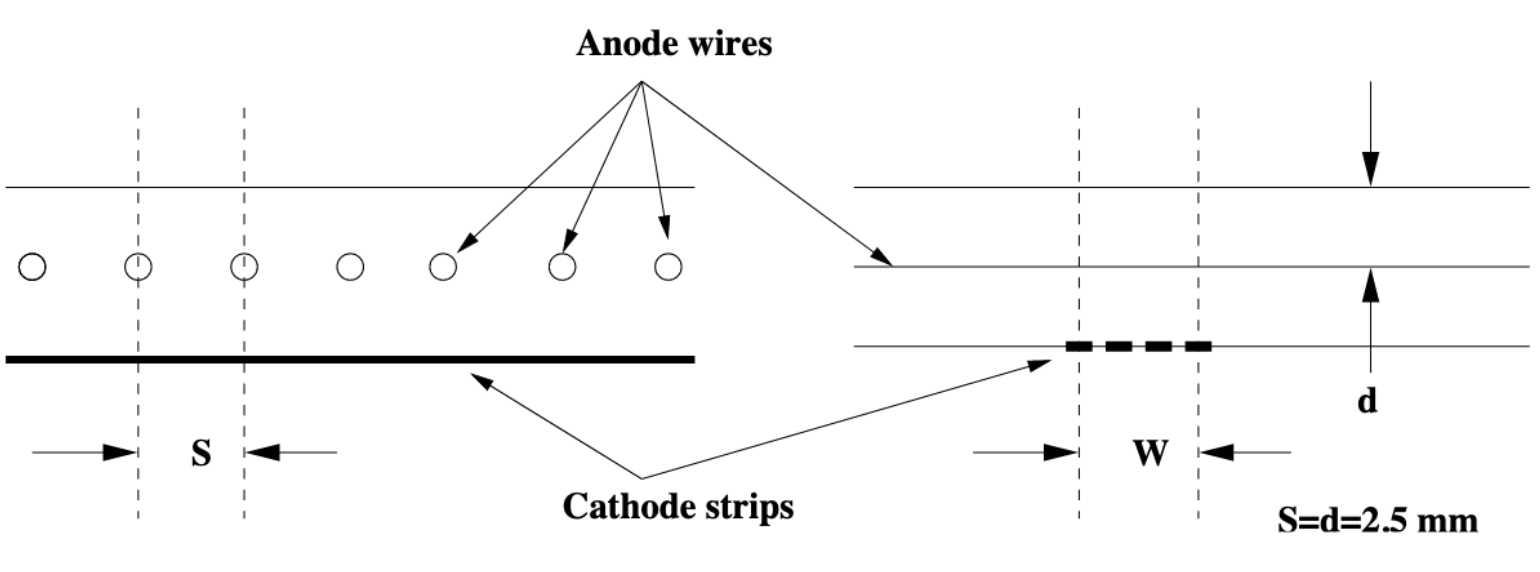
\includegraphics[width=.6\textwidth]{figures/ch3-LHC-ATLAS/CSC_Diagram.png}\hspace{0.3cm}
    }
    \subfloat[]{
    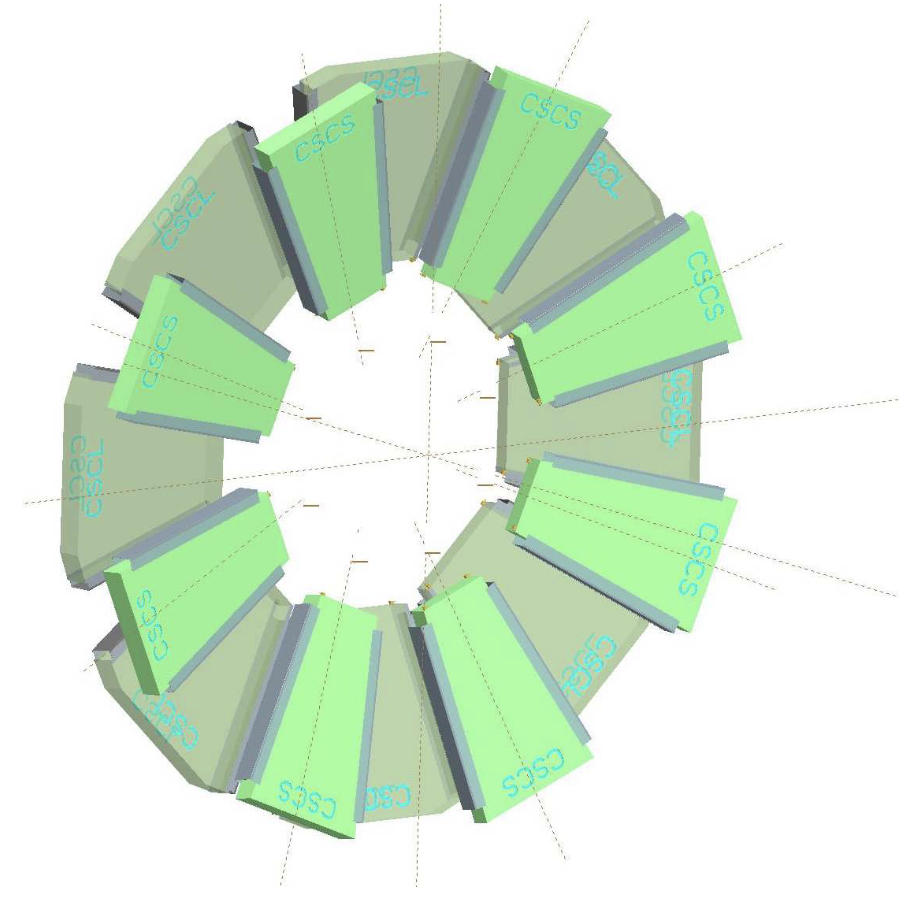
\includegraphics[width=.35\textwidth]{figures/ch3-LHC-ATLAS/CSC_wheelstruct.png}
    }
    \caption{(a) The cross-section of the CSC chamber in the wire length direction, and (b) the CSC End-Cap wheel structure with small and large chambers~\cite{PERF-2007-01}.}
    \label{fig:csc_struct}
\end{figure}
Signal readout is accomplished using dual cathode strip planes. By running one plane perpendicular to the anode wires and the other parallel to them, the system simultaneously registers coordinates in the non-bending and bending planes.

The physical layout and internal structure of the CSCs are mapped in Figure~\ref{fig:csc_struct}. Because they must endure the highest particle fluxes, CSC modules are strategically mounted only on the innermost end-cap station, covering the $2 < |\eta| < 2.7$ geometry. A complete CSC wheel integrates eight large and eight small chamber units. With four independent CSC planes housed in every chamber, the system easily extracts four distinct positional measurements across both $\phi$ and $\eta$. The defining technical specifications for the CSCs are compiled in Table~\ref{tab:summary_CSC}.

Along the non-bending vector, the CSCs provide a spatial resolution of roughly 5~mm~\cite{PERF-2007-01}. Beyond spatial tracking, CSCs deliver a highly precise timing resolution of around 7~ns. They are also highly immune to neutron background scatter and possess an excellent capacity for separating closely adjacent tracks.

\begin{table}[!htbp]
    \centering
    \begin{tabular}{l|c}
        \hline\hline
        \textbf{CSC Parameter} & \textbf{Value} \\
        \hline
        Gas mixture & Ar/CO$_2$ (80\%/20\%) \\
        Operating voltage & 1900 V \\
        % Wire material & W/Re (97\%/3\%); 3\% gold plating \\
        Gas pressure & 1 atm \\
        Gas gain & $6\times10^4$ \\
        Number of planes/chamber & 4 \\
        Anode wire diameter & 30 $\mu$m \\
        Anode wire pitch & 2.50 mm \\
        Distance anode wires - cathode strips & 2.50 mm \\
        Average resolution of each plane & 60 $\mu$m \\
        \hline\hline
    \end{tabular}
    \caption{Summary of important parameters of the Cathode Strip Chamber.}
    \label{tab:summary_CSC}
\end{table}

\noindent\textbf{Resistive Plate Chambers (RPCs)} \\
Tasked with generating rapid trigger decisions throughout the barrel zone, the RPC system is organized into three cylindrical layers wrapping coaxially around the beam pipe. Taking advantage of the substantial geometric gap (lever arm) between the inner two layers and the outer third layer, the RPC framework effortlessly executes a high-$p_T$ trigger algorithm (for targets between 9 and 35~GeV), while the inner double-layer handles low-$p_T$ triggers (6 to 9~GeV). This built-in multi-layer redundancy supports a rigorous coincidence logic that significantly boosts overall trigger reliability by filtering out false tracks caused by random noise.

Fundamentally, RPCs are wire-less, gas-filled parallel-plate sensors. The 2~mm gap separating the parallel plates is heavily electrified, creating a uniform 4.9~kV/mm electric field. Inside the gap, the detector relies on a C$_2$H$_2$F$_4$/Iso-C$_4$H$_{10}$/SF$_6$ (94.7/5/0.3) gas blend. An anatomical look at an RPC module and its integration into the broader station is available in Figure~\ref{fig:rpc_struct}.

\begin{figure}[!htbp]
    \centering
    \subfloat[]{
    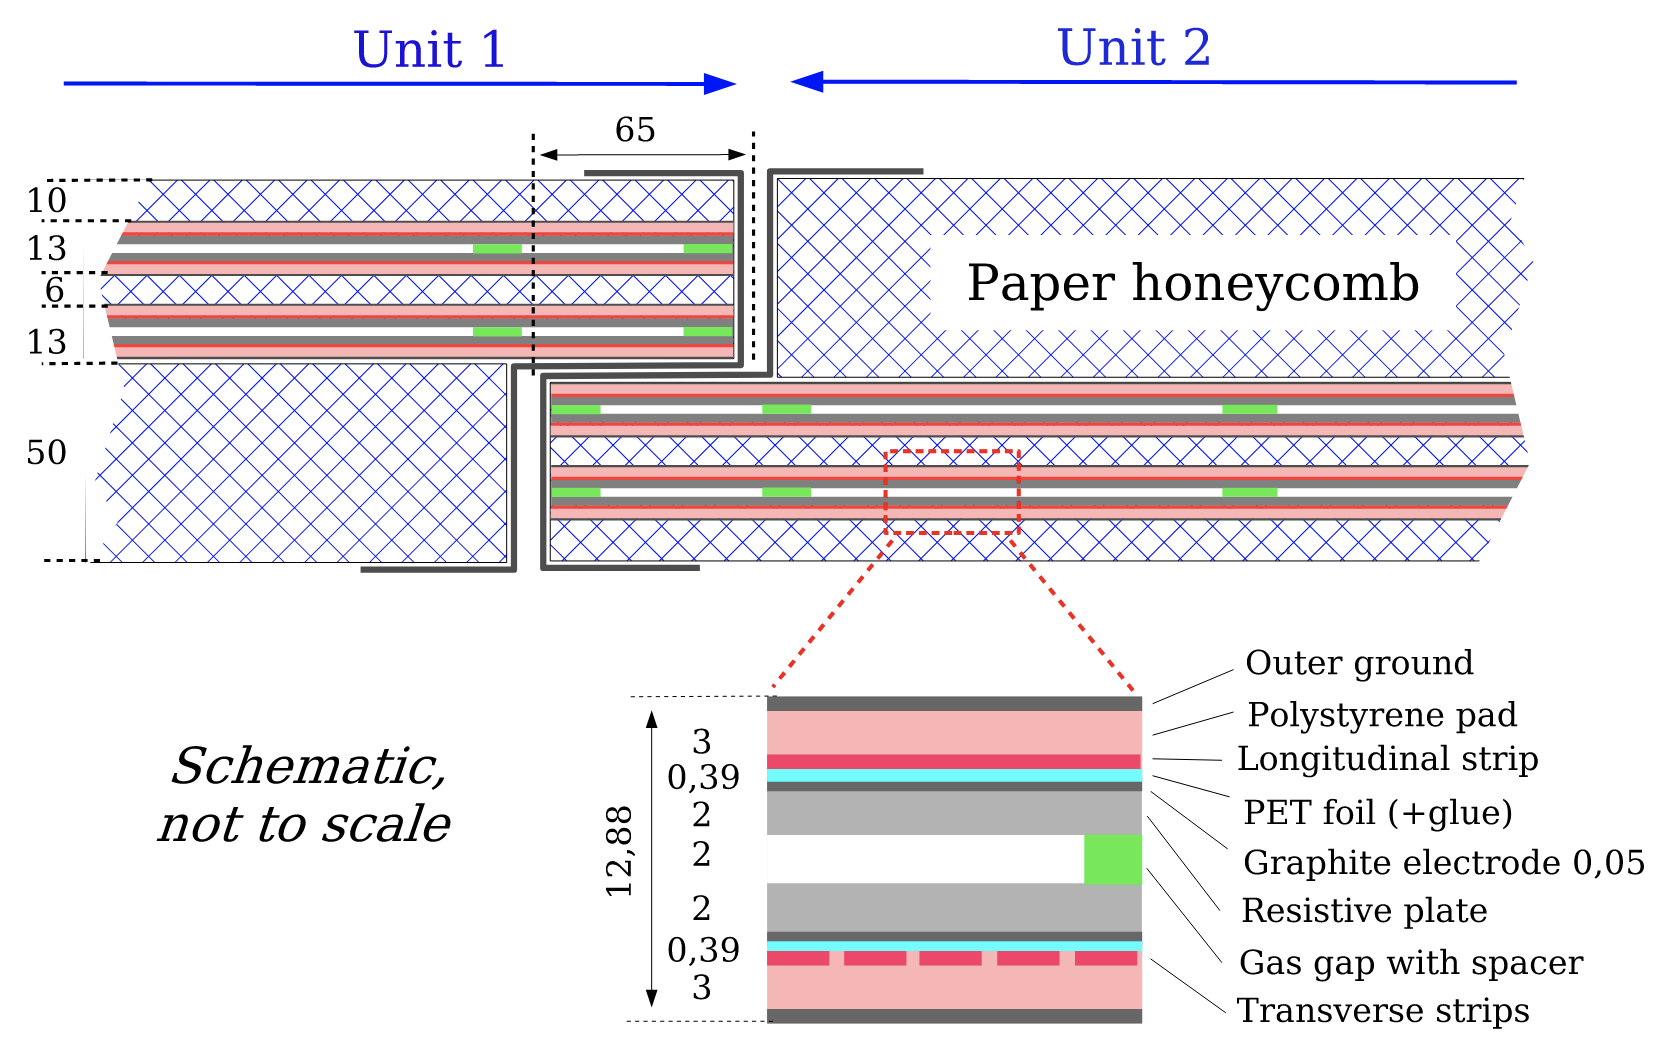
\includegraphics[width=.45\textwidth]{figures/ch3-LHC-ATLAS/RPC_Diagram.png}
    \label{subfig:rpc_diag}
    }
    \qquad
    \subfloat[]{
    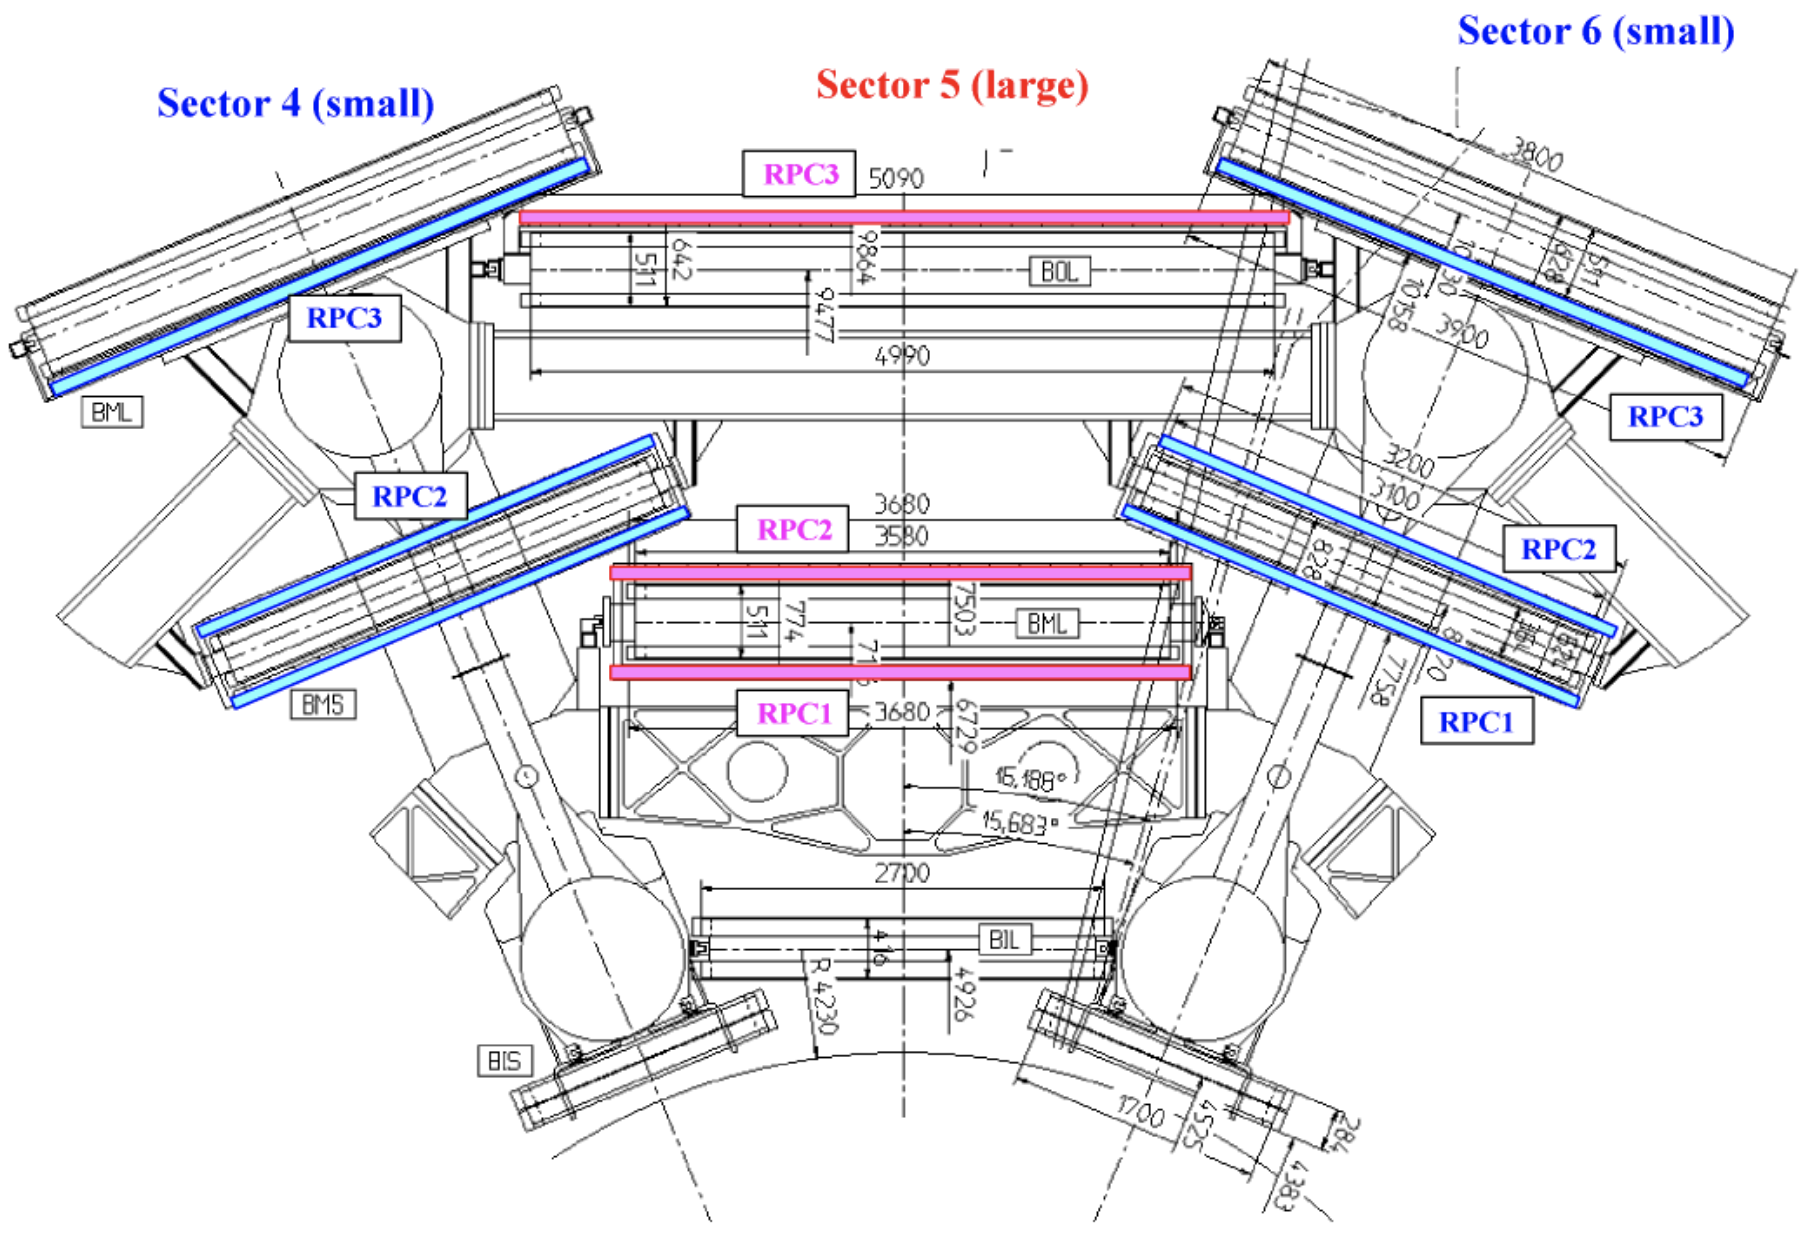
\includegraphics[width=.45\textwidth]{figures/ch3-LHC-ATLAS/RPC_stations.png}
    \label{subfig:rpc_mechstruct}
    }
    \caption{(a) The cross-section of an RPC with two units joined to form a chamber~\cite{PERF-2007-01}, and (b) the RPC stations with respect to the MDT station positions~\cite{PERF-2007-01}.}
    \label{fig:rpc_struct}
\end{figure}

\begin{table}[!htbp]
    \centering
    \begin{tabular}{c|c}
        \hline\hline
        \textbf{Parameter} & \textbf{Value} \\
        \hline
        Gas mixture & C$_2$H$_2$F$_4$/i-C$_4$H$_10$/SF$_6$ (94.7\%/5\%/0.3\%) \\
        Operating voltage & 4.9 kV/mm \\
        Resistive plate material & Plastic laminate \\
        Resistive plate thickness & 1.8 mm \\
        Volume resistivity & $10^{10}\Omega\cdot\text{cm}$ \\
        Gas gap thickness & 2 mm \\
        Gas pressure & 5 mbar \\
        Average single-hit resolution & 5-10 mm \\
        \hline\hline
    \end{tabular}
    \caption{Summary of important parameters of the Resistive Plate Chamber.}
    \label{tab:summary_RPC}
\end{table}

\noindent\textbf{Thin Gap Chambers (TGCs)} \\
In the end-cap zones, the crucial muon trigger functionality is driven by the TGCs. By accurately measuring the azimuthal track coordinate, the TGCs perfectly complement the radial data provided by the companion MDT arrays. Specifically, the innermost muon station houses two layers of TGCs, while the middle end-cap station (also known as the EM wheels) is packed with seven TGC layers.

The primary inner layer (the I layer) is physically divided into two concentric zones: the forward (FI) section and the end-cap (EI) section. United, these sections comprise the ``Small Wheel.'' To build out the detection volume, the TGC framework utilizes two doublets (totaling four layers) for the inner station, and an assembly of two doublets flanking a triplet (seven layers) for the middle station.

Technically, a TGC is a multiwire proportional chamber characterized by an incredibly tight wire-to-cathode gap (1.4~mm), which is actually smaller than the distance separating adjacent wires (1.8~mm). It operates using a highly quenching 55\%/45\% mixture of CO$_2$ and n-pentane. This combination of a potent electric field and ultra-compact wire spacing yields an astonishing timing resolution; a staggering 99\% of all signals are successfully captured within the strict 25~ns bunch-crossing window. The internal layout of a typical TGC is showcased in Figure~\ref{fig:tgc_struct}.

\begin{figure}[!htbp]
\centering
\subfloat[]{
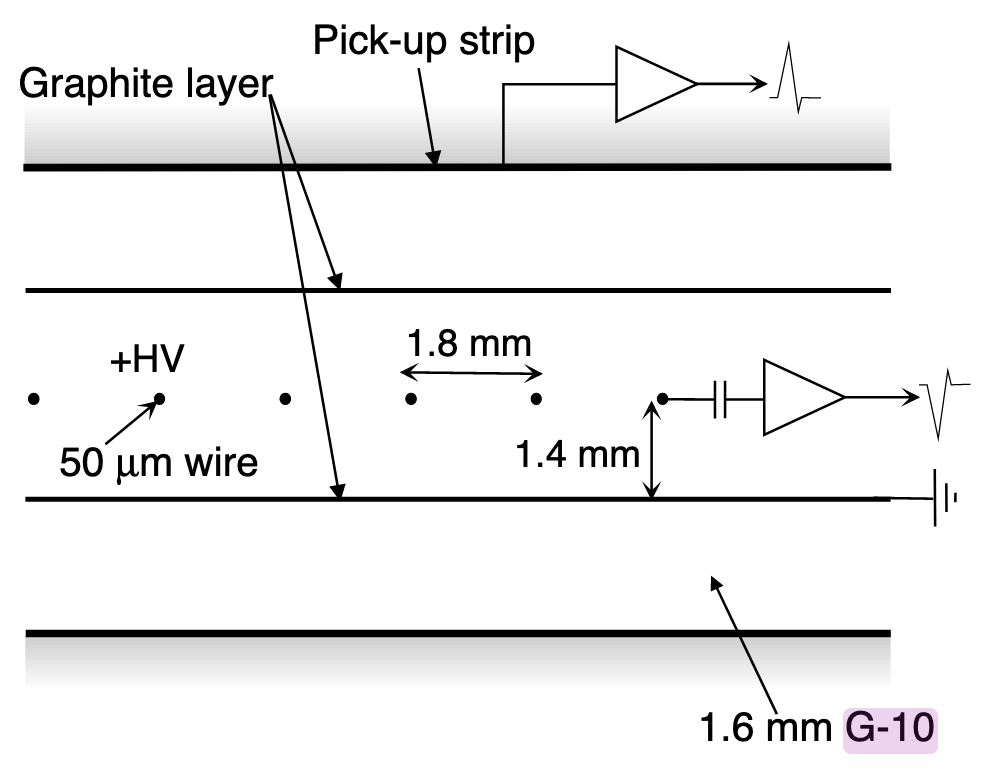
\includegraphics[width=.45\textwidth]{figures/ch3-LHC-ATLAS/TGC_Diagram.png}
\label{subfig:tgc_diag}
}
\qquad
\subfloat[]{
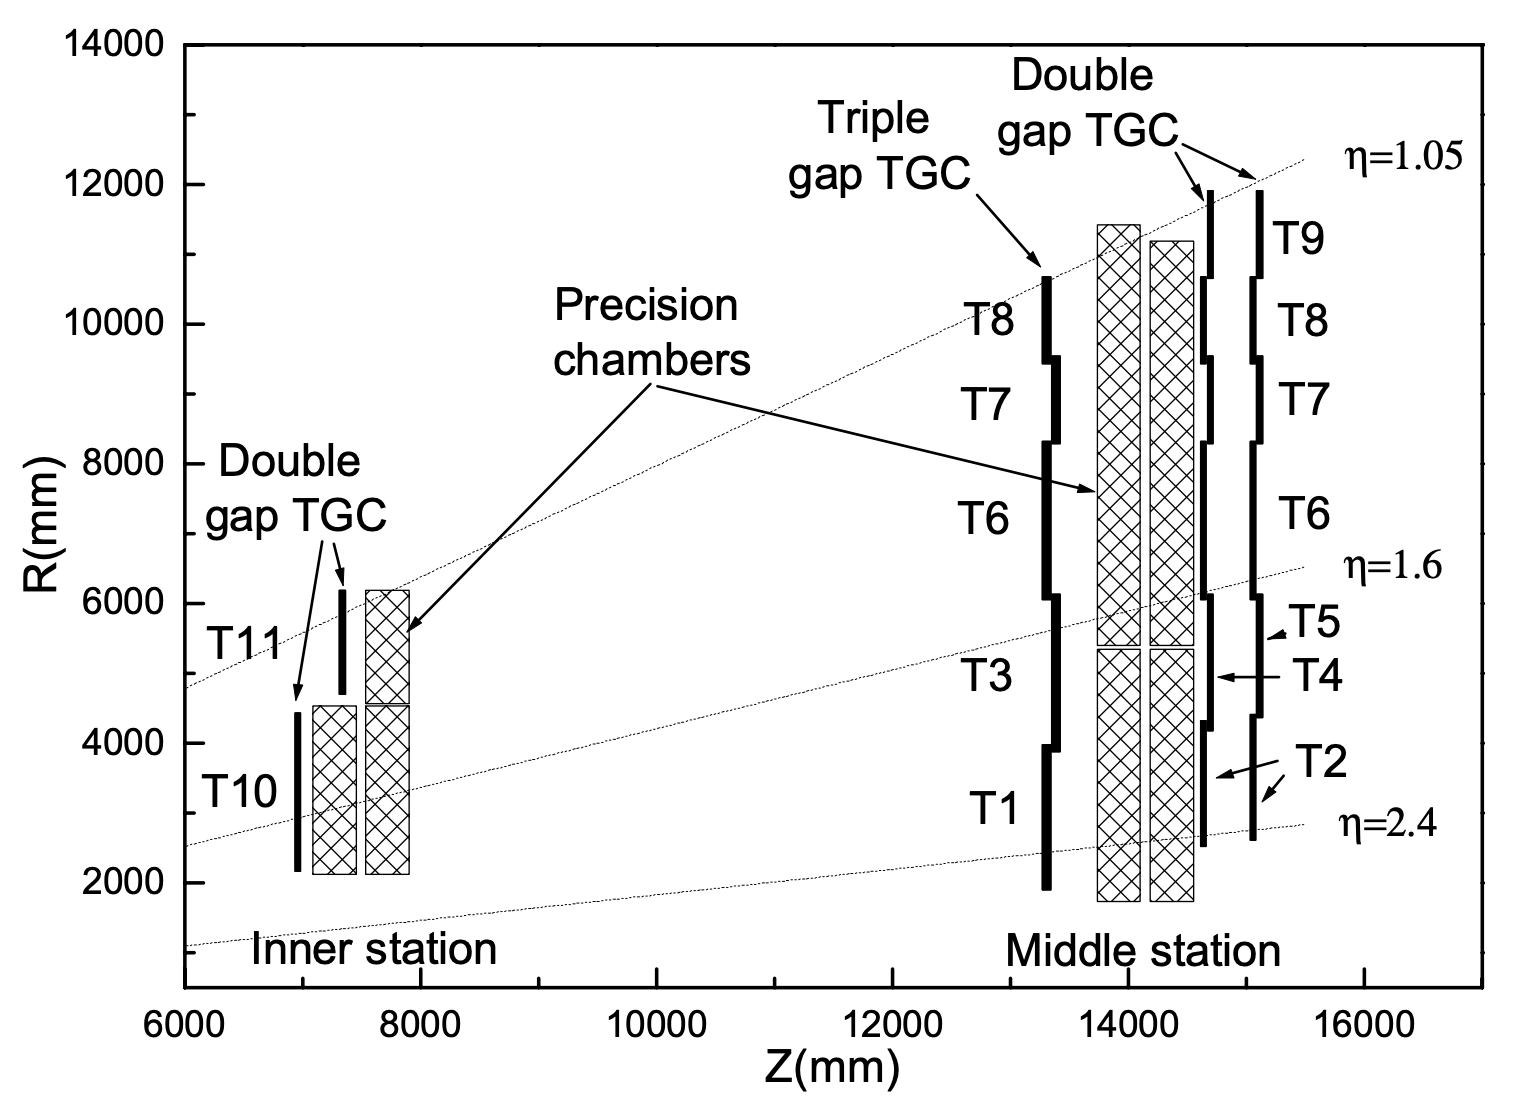
\includegraphics[width=.45\textwidth]{figures/ch3-LHC-ATLAS/TGC_Inner_Middle_Layers.png}
\label{subfig:tgc_layers}
}
\caption{(a) The cross-section view of the TGC detector~\cite{PERF-2007-01}, and (b) different TGC layers in the End-Cap (I layer and Big Wheels)~\cite{PERF-2007-01}.}
\label{fig:tgc_struct}
\end{figure}

\begin{table}[!htbp]
    \centering
    \begin{tabular}{c|c}
        \hline\hline
        \textbf{Parameter} & \textbf{Value} \\
        \hline
        Gas mixture & CO$_2$/n-C$_5$H$_{12}$ (55\%/45\%) \\
        Operating voltage & 200 V \\
        Gas gap & 2.8 $\pm$ 0.10 mm \\
        Gas pressure & 3 bar \\
        Gas amplification & $3\times10^{5}$ \\
        Wire pitch & 1.8 $\pm$ 0.05 mm \\
        Wire diameter & 50 $\mu$m \\
        Average single-hit resolution & 1-2 mm \\
        \hline\hline
    \end{tabular}
    \caption{Summary of important parameters of the Thin Gap Chamber.}
    \label{tab:summary_TGC}
\end{table}

Following the conclusion of Run~2, the Muon Spectrometer was the subject of an intense Phase-I modernization program. The most visible change was the complete retirement of the old end-cap Small Wheel (originally built from MDT and CSC modules) in favor of the New Small Wheel (NSW). The NSW embraces cutting-edge small-strip Thin Gap Chambers (sTGC) and Micromegas (MM) technologies~\cite{ATLAS-NSW-TDR}. Thanks to this overhaul, the MS is fully prepared to function reliably amidst the fierce particle backgrounds generated by the LHC's luminosity increases.

%%%%%%%%%%%%%%%%%%%%%%%%%%%%%%%%%%%%%%%%%%%
\subsection{Magnet System}

To accurately determine the momentum and charge of charged particles, the ATLAS experiment relies heavily on its sophisticated magnet system~\cite{ATLAS-TDR-06}. This massive installation is divided into four primary components: dual end-cap toroid magnets, a central solenoid, and a colossal barrel toroid (depicted in Figure~\ref{fig:atlas-magnet}).

\begin{figure}[!htbp]
\centering
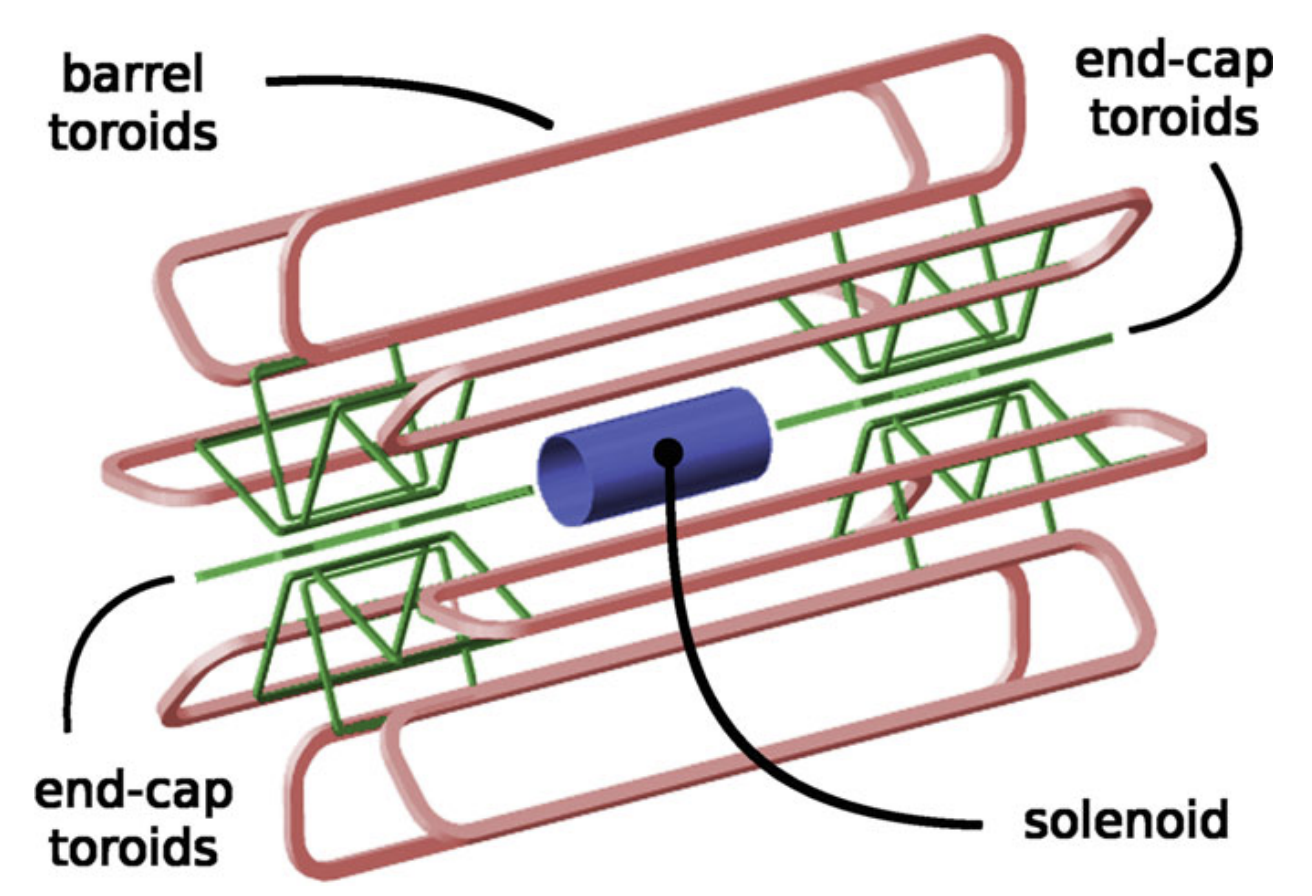
\includegraphics[width=0.65\textwidth]{figures/ch3-LHC-ATLAS/ATLAS_magnet_2.png}
\caption{The ATLAS solenoid (center) and toroidal magnet system~\cite{Bryngemark2017}.}
\label{fig:atlas-magnet}
\end{figure}

Tasked with bending the paths of charged particles within the Inner Detector (ID) to permit momentum extraction, the central solenoid establishes a robust 2~T axial magnetic field. Weighing approximately 5 tonnes, the solenoid structure features a 2.4~m diameter and extends 5.3~m in length. Crucially, its wall thickness (a mere 4.5~cm) was heavily optimized to minimize material obstruction in front of the electromagnetic calorimeter, ensuring that passing particles suffer negligible energy interference. Spooled with roughly 9~km of superconducting cable, the solenoid holds roughly 38~MJ of stored energy and operates at a baseline current of 7.73~kA.

Outwardly, the two end-cap toroids and the barrel toroid are responsible for generating the magnetic curvature necessary for the muon spectrometer. Built from eight gigantic, symmetrically positioned superconducting coils, the barrel toroid alone stores an immense 1.08~GJ of magnetic energy. Complementing the barrel, the two end-cap toroids sit at the detector's extremities, each projecting a formidable 4~T field. Tipping the scales at 240 tonnes apiece, each end-cap unit holds about 0.25~GJ of energy. To maintain their superconducting state, all toroid magnets are chilled to roughly 4.7~K and operate using an intense 20.5~kA nominal current.

%%%%%%%%%%%%%%%%%%%%%%%%%%%%%%%%%%%
\subsection{Trigger and Data Acquisition System}
\label{sec:ATLAS_TDAQ}

Proton-proton bunches cross at a frequency of 40~MHz within the LHC. During Run~2, depending on fluctuating instantaneous luminosity profiles, each individual 25~ns bunch crossing triggered an average of 10 to 60 simultaneous proton-proton collisions~\cite{DAPR-2018-01}. This pile-up effect generates a torrential flood of raw data. Because logging this entire data stream to permanent storage is technologically and economically impossible, ATLAS relies on a highly efficient trigger and data acquisition (TDAQ) system to selectively preserve only the most physically compelling events.

Considering an average event size of approximately 1.7~MB during Run~2~\cite{ATL-DAQ-PROC-2015-064}, attempting to record data at the raw 40~MHz crossing rate would demand an incomprehensible bandwidth. To combat this, the trigger system acts as a multi-tier filter, radically slashing the event rate step by step. By the time the data clears the High-Level Trigger (HLT) phase, the acceptance rate is throttled down to roughly 1~kHz, which cleanly matches a manageable recording bandwidth of about 1.2~GB/s~\cite{DAPR-2018-01}.

\begin{figure}[!htbp]
\centering
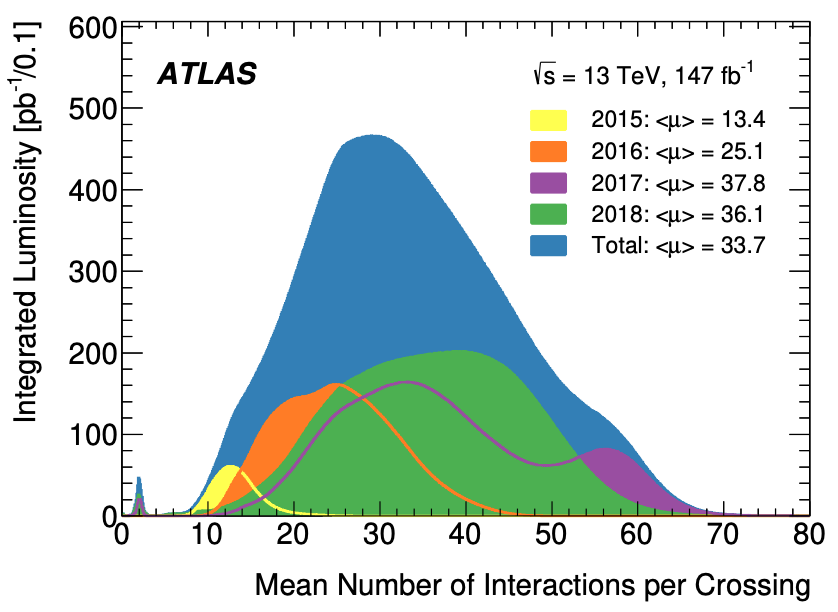
\includegraphics[width=0.6\textwidth]{figures/ch3-LHC-ATLAS/ATLAS_meaninter_perbunch_Run2.png}
\caption{Average number of interactions per bunch crossing for the dataset used in Run~2~\cite{DAPR-2018-01}.}
\label{fig:bunch_inter_Run2}
\end{figure}

The ATLAS TDAQ system effortlessly orchestrates data recording, online event filtration, and real-time processing. For the duration of Run~2, the framework utilized a streamlined two-level trigger hierarchy~\cite{TRIG-2016-01}. A high-level schematic of this data flow is presented in Figure~\ref{fig:ATLAS_Trigger}.

\begin{figure}[!htbp]
\centering
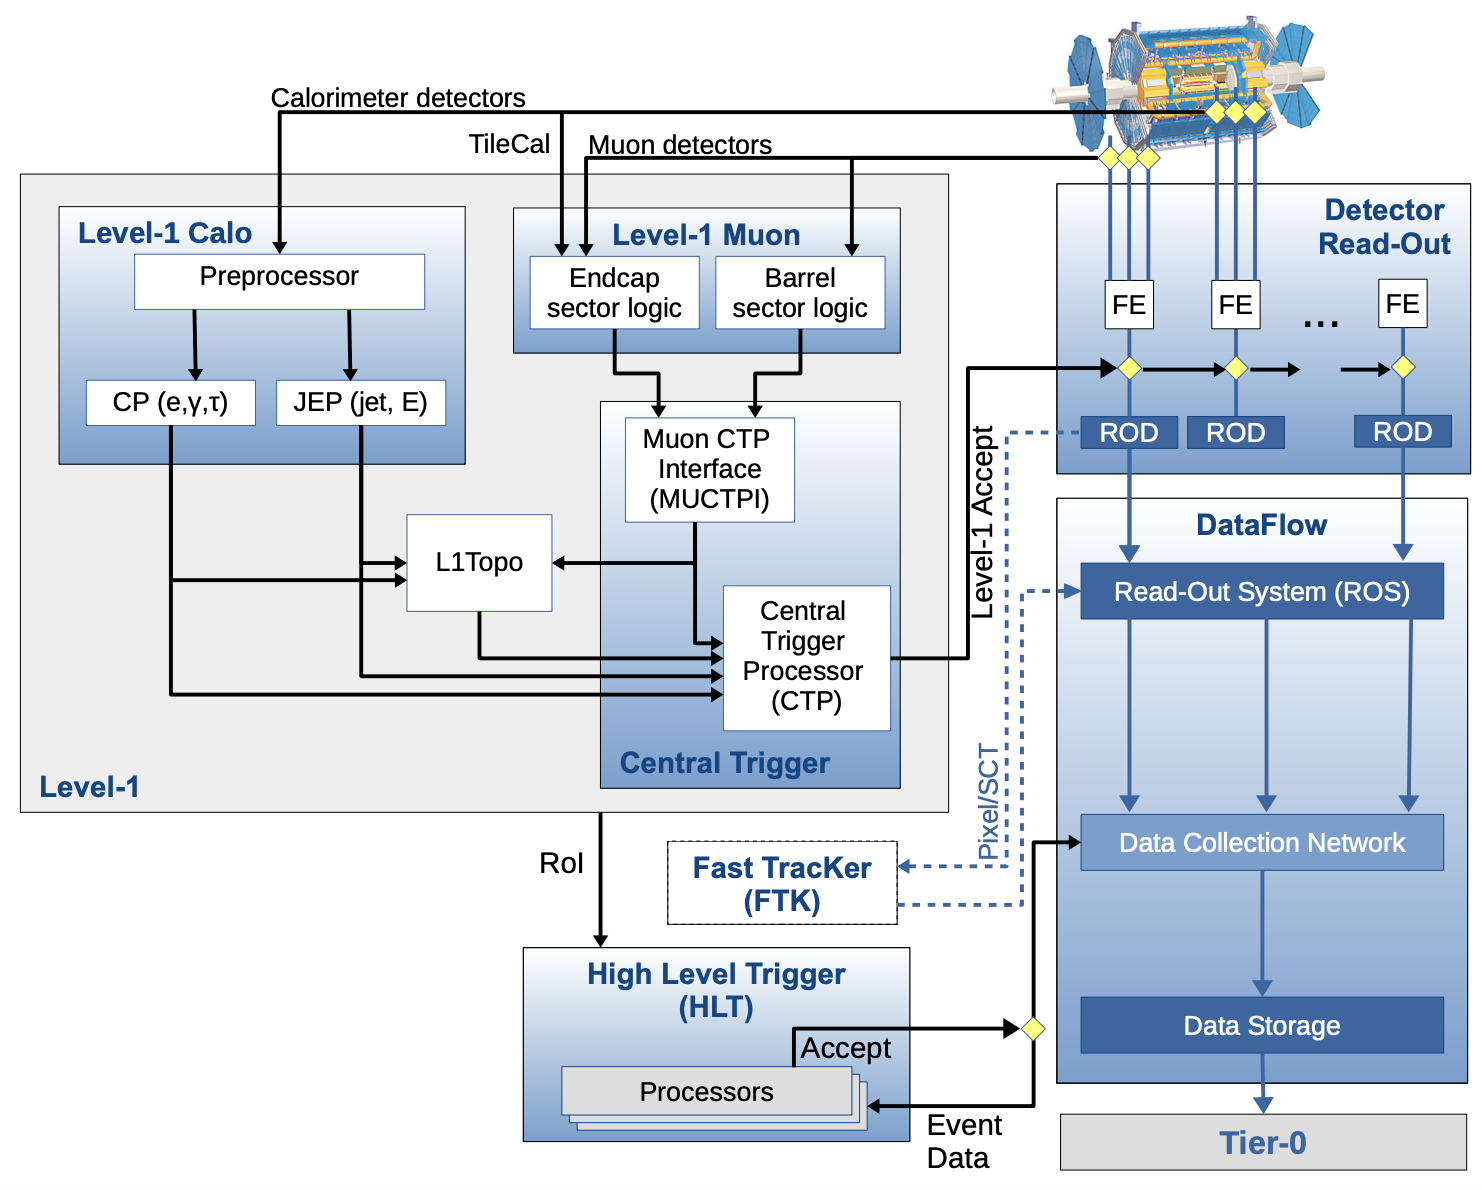
\includegraphics[width=0.95\textwidth]{figures/ch3-LHC-ATLAS/ATLAS_Trigger.png}
\caption{The ATLAS TDAQ system during Run~2, showing the trigger components as well as detector read-out and data flow~\cite{ATLAS_Run2_TDAQ2020}.}
\label{fig:ATLAS_Trigger}
\end{figure}

Fundamentally, the ATLAS trigger pipeline exists to isolate specific events that exhibit the hallmarks of rare or significant physics, specifically targeting high-$p_\text{T}$ anomalies spawned by hard-scattering collisions. This massive filtration effort is executed sequentially via the Level-1 (L1) hardware trigger and the software-driven High-Level Trigger (HLT), detailed below.

\noindent\textbf{1) Level-1 Trigger}  \\
Executing rapid, hardware-level logic checks, the Level-1 (L1) trigger mines coarse data feeds from the muon chambers and calorimeters to instantly decide if an event warrants further inspection~\cite{ATLAS-TDR-12}.

\begin{itemize}

\item Taking its cues from the calorimeter arrays, the Level-1 calorimeter trigger (L1Calo) springs into action. Raw analog signals are first intercepted, digitized, and calibrated by a dedicated pre-processor. These clean signals are simultaneously broadcast to the Jet/Energy-sum Processor (JEP) and the Cluster Processor (CP). The CP's role is to flag potential $\tau$-leptons, photons, and electrons that breach predefined energy thresholds. Simultaneously, the JEP calculates macro-level event parameters like missing transverse energy and hunts for potential jet clusters. To prevent minor energy baseline drifts from corrupting the missing energy calculations, the firmware routinely runs an aggressive pedestal correction protocol.

\item Utilizing tracking hits from the Thin Gap Chambers (TGCs) and Resistive Plate Chambers (RPCs) discussed in Section~\ref{chap:MS}, the Level-1 muon trigger (L1Muon) executes track matching. To strictly filter out background noise or stray particles that did not originate from the central collision vertex, the system enforces rigid coincidence mandates across several distinct muon stations. Specifically within the end-caps during Run~2, the L1Muon logic required overlapping signals from both inner and outer TGC modules, frequently paired with coincidental hits from the adjacent tile calorimeter.

\end{itemize}

The ultimate L1 validation verdict is finalized by the Central Trigger Processor (CTP), which merges the diagnostic outputs from both the L1Muon and L1Calo pipelines. The CTP also factors in supplementary telemetry from specialized detectors like the Zero Degree Calorimeter (ZDC), LUCID, and the Minimum Bias Trigger Scintillators (MBTS). Furthermore, the CTP orchestrates complex dead-time protocols to restrict the absolute number of accepted events within tight timeframes, guaranteeing that electronic readout windows never overlap.

The criteria for L1 event selection are highly flexible: they can hinge on complex topological rules (like angular geometry or invariant mass), object tallies (requiring multiple muons above a specific momentum), or broad global metrics (like raw calorimeter energy sums). Operating at a remarkably fast latency of roughly 2.5~$\mu$s, the L1 network effectively crushes the incoming 40~MHz event barrage down to a ceiling of 100~kHz, aligning perfectly with the hardware readout limits.

Once the L1 trigger approves an event, the local front-end (FE) electronics extract the raw data from the detector modules and push it to the ReadOut Drivers (RODs) for initial formatting. This packaged data stream is subsequently warehoused in the ReadOut System (ROS). The ROS buffers these fragments until the HLT officially requests them. As a final output, the L1 trigger plots specific spatial Regions of Interest (RoIs) defined by $\phi$ and $\eta$, handing these coordinates over to focus the HLT's reconstruction algorithms.

\noindent\textbf{2) High-Level Trigger} \\ 
Acting as the final filtration tier, the High-Level Trigger (HLT) relies entirely on sophisticated software protocols executed across a massive computing farm~\cite{ATLAS-TDR-16}. Initially deploying rapid reconstruction heuristics, the HLT subsequently follows up with rigorous, CPU-intensive algorithms that closely mirror the precision routines used during ultimate offline analysis.

HLT algorithms excel at targeted feature extraction. Depending on the exact physics object being scrutinized, the HLT might request targeted data strictly from the pre-defined L1 RoIs, or it might demand a global sweep of the entire detector (for instance, when calculating missing transverse momentum). Throughout the Run~2 campaign, the HLT successfully throttled the incoming 100~kHz L1 feed down to an average final acceptance rate of 3~kHz, capping the external data throughput at an easily manageable 6~GB/s.

Events that survive the rigorous HLT gauntlet are shuttled by the Sub-Farm Output (SFO) network into permanent data storage. From there, the files are systematically exported directly to the CERN Tier-0 computing grid, where comprehensive offline analysis and full event reconstruction commence in earnest~\cite{ATLAS-TDR-17}.

\begin{table}[!htbp]
    \centering
    \begin{tabular}{c|c|c|c|c}
        \hline\hline
        \textbf{LHC Period} & \textbf{Trigger} & \textbf{Incoming event rate} & \textbf{Outgoing rate \& Bandwidth} & \textbf{Reduction factor} \\ 
        \hline
        \multirow{2}{*}{Run 2} & Level 1 & 40 MHz  & 100 kHz ; $\sim$160 GB/s & 400 \\
                               & HLT     & 100 kHz & 1 kHz ; $\sim$1.2 GB/s   & 100 \\
        \hline
        \multirow{2}{*}{Run 3} & Level 1 & 40 MHz  & 100 kHz ; $\sim$300 GB/s & 400 \\
                               & HLT     & 100 kHz & 3 kHz ; $\sim$6.0 GB/s   & $\sim$33 \\
        \hline\hline
    \end{tabular}
    \caption{Summary of event rates and reduction factors in the ATLAS trigger system comparing LHC Run 2~\cite{ATLAS-Run2-Trigger} and Run 3~\cite{ATLAS-Run3-Trigger} operations.}
    \label{tab:summary_trigger}
\end{table}